\documentclass[runningheads]{llncs}
\usepackage[T1]{fontenc}
\usepackage{booktabs}

\usepackage{amsmath}
\usepackage{amssymb}
\usepackage{hyperref}
\usepackage{algorithm}
\usepackage{algpseudocode}
\usepackage{tikz}
\usetikzlibrary{shapes, arrows.meta, positioning, calc, fit, backgrounds}

% -------------------------------------------------------------------------
% EMBEDDED BIBLIOGRAPHY
% ----------------------------------------------------------------------
% -------------------------------------------------------------------------
% EMBEDDED BIBLIOGRAPHY
% -------------------------------------------------------------------------
\usepackage{filecontents}
\begin{filecontents}{references.bib}
@inproceedings{rerum2024,
  title={Rankability-enhanced Revenue Uplift Modeling Framework for Online Marketing},
  author={He, Bowei and Weng, Yunpeng and Tang, Xing and Cui, Ziqiang and Sun, Zexu and Chen, Liang and He, Xiuqiang and Ma, Chen},
  booktitle={Proceedings of the 30th ACM SIGKDD Conference on Knowledge Discovery and Data Mining},
  year={2024},
  publisher={ACM}
}

@inproceedings{dfcl2023,
  title={Decision Focused Causal Learning for Direct Counterfactual Marketing Optimization},
  author={Zhou, Hao and Huang, Rongxiao and Li, Shaoming and Jiang, Guibin and Zheng, Jiaqi and Cheng, Bing and Lin, Wei},
  booktitle={Proceedings of the 30th ACM SIGKDD Conference on Knowledge Discovery and Data Mining},
  year={2024},
  publisher={ACM}
}

@inproceedings{efin2023,
  title={Explicit Feature Interaction-aware Uplift Network for Online Marketing},
  author={Liu, Dugang and Tang, Xing and Gao, Han and Lyu, Fuyuan and He, Xiuqiang},
  booktitle={Proceedings of the 29th ACM SIGKDD Conference on Knowledge Discovery and Data Mining},
  year={2023},
  publisher={ACM}
}

@inproceedings{tppum2025,
  title={Temporal Uplift Modeling for Online Marketing},
  author={Zhang, Xin and Wang, Kai and Wang, Zengmao and Du, Bo and Zhao, Shiwei and Wu, Runze and Shen, Xudong and Lv, Tangjie and Fan, Changjie},
  booktitle={Proceedings of the 30th ACM SIGKDD Conference on Knowledge Discovery and Data Mining},
  year={2024},
  publisher={ACM}
}

@inproceedings{sun2025robust,
  title={Robust Uplift Modeling with Large-Scale Contexts for Real-time Marketing},
  author={Sun, Zexu and Han, Qiyu and Zhu, Minqin and Gong, Hao and Liu, Dugang and Ma, Chen},
  booktitle={Proceedings of the 31st ACM SIGKDD Conference on Knowledge Discovery and Data Mining},
  year={2025},
  publisher={ACM},
  doi={10.1145/3690624.3709293}
}

@article{hillstrom2008,
  title={The MineThatData e-mail analytics and data mining challenge},
  author={Hillstrom, Kevin},
  journal={MineThatData blog},
  year={2008}
}

@article{rzepakowski2012,
  title={Decision trees for uplift modeling with single and multiple treatments},
  author={Rzepakowski, Piotr and Jaroszewicz, Szymon},
  journal={Knowledge and Information Systems},
  volume={32},
  pages={303--327},
  year={2012}
}

@inproceedings{shalit2017estimating,
  title={Estimating individual treatment effect: generalization bounds and algorithms},
  author={Shalit, Uri and Johansson, Fredrik D and Sontag, David},
  booktitle={International Conference on Machine Learning},
  pages={3076--3085},
  year={2017},
  organization={PMLR}
}

@inproceedings{shi2019adapting,
  title={Adapting neural networks for the estimation of treatment effects},
  author={Shi, Claudia and Blei, David and Veitch, Victor},
  booktitle={Advances in neural information processing systems},
  volume={32},
  year={2019}
}

@inproceedings{kunzel2019metalearners,
  title={Metalearners for estimating heterogeneous treatment effects using machine learning},
  author={K{\"u}nzel, S{\"o}ren R and Sekhon, Jasjeet S and Bickel, Peter J and Yu, Bin},
  booktitle={Proceedings of the national academy of sciences},
  volume={116},
  number={10},
  pages={4156--4165},
  year={2019}
}

@article{su2009,
  title={Subgroup Analysis via Recursive Partitioning},
  author={Su, Xiaogang and Tsai, Chih-Ling and Wang, Hansi and Nickerson, David M. and Li, Bogong},
  journal={Journal of Machine Learning Research},
  volume={10},
  number={2},
  pages={141--158},
  year={2009},
  publisher={JMLR. org}
}

@article{rubin2005causal,
  title={Causal inference using potential outcomes: Design, modeling, decisions},
  author={Rubin, Donald B},
  journal={J. Amer. Statist. Assoc.},
  volume={100},
  number={469},
  pages={322--331},
  year={2005}
}

@article{calder2003feature,
  title={Feature interaction: a critical review and considered forecast},
  author={Calder, Muffy and Kolberg, Mario and Magill, Evan H and Reiff-Marganiec, Stephan},
  journal={Computer Networks},
  volume={41},
  number={1},
  pages={115--141},
  year={2003}
}

@inproceedings{wu2023stable,
  title={Stable estimation of heterogeneous treatment effects},
  author={Wu, Anpeng and Kuang, Kun and Xiong, Ruoxuan and Li, Bo and Wu, Fei},
  booktitle={International Conference on Machine Learning},
  pages={37496--37510},
  year={2023},
  organization={PMLR}
}

@article{athey2019estimating,
  title={Estimating treatment effects with causal forests: An application},
  author={Athey, Susan and Wager, Stefan},
  journal={Observational studies},
  volume={5},
  number={2},
  pages={37--51},
  year={2019}
}

@inproceedings{liu2023unite,
  title={UniTE: A Unified Treatment Effect Estimation Method for One-sided and Two-sided Marketing},
  author={Liu, Runshi and Hou, Zhipeng},
  booktitle={Proceedings of the 32nd ACM International Conference on Information and Knowledge Management},
  pages={1472--1481},
  year={2023}
}

@article{gubela2020response,
  title={Response transformation and profit decomposition for revenue uplift modeling},
  author={Gubela, Robin M and Lessmann, Stefan and Jaroszewicz, Szymon},
  journal={European Journal of Operational Research},
  volume={283},
  number={2},
  pages={647--661},
  year={2020},
  publisher={Elsevier}
}

@inproceedings{DBLP:conf/amcis/GubelaL20,
  author       = {Robin Marco Gubela and
                  Stefan Lessmann},
  editor       = {Bonnie Brinton Anderson and
                  Jason Thatcher and
                  Rayman D. Meservy and
                  Kathy Chudoba and
                  Kelly J. Fadel and
                  Sue Brown},
  title        = {Interpretable Multiple Treatment Revenue Uplift Modeling},
  booktitle    = {26th Americas Conference on Information Systems, {AMCIS} 2020, Virtual
                  Conference, August 15-17, 2020},
  publisher    = {Association for Information Systems},
  year         = {2020},
  url          = {https://aisel.aisnet.org/amcis2020/data\_science\_analytics\_for\_decision\_support/data\_science\_analytics\_for\_decision\_support/18},
  timestamp    = {Mon, 27 Jul 2020 19:07:22 +0200},
  biburl       = {https://dblp.org/rec/conf/amcis/GubelaL20.bib},
  bibsource    = {dblp computer science bibliography, https://dblp.org}
}

@article{wang2019deep,
  title={A deep probabilistic model for customer lifetime value prediction},
  author={Wang, Xiaojing and Liu, Tianqi and Miao, Jingang},
  journal={arXiv preprint arXiv:1912.07753},
  year={2019}
}

@article{devriendt2020learning,
  title={Learning to rank for uplift modeling},
  author={Devriendt, Floris and Van Belle, Jente and Guns, Tias and Verbeke, Wouter},
  journal={IEEE Transactions on Knowledge and Data Engineering},
  volume={34},
  number={10},
  pages={4888--4904},
  year={2020},
  publisher={IEEE}
}

@article{abdi2007kendall,
  title={The Kendall rank correlation coefficient},
  author={Abdi, Herv{\'e}},
  journal={Encyclopedia of Measurement and Statistics. Sage, Thousand Oaks, CA},
  pages={508--510},
  year={2007}
}

@inproceedings{guo2017deepfm,
  title={DeepFM: A factorization-machine based neural network for CTR prediction},
  author={Guo, Huifeng and Tang, Ruiming and Ye, Yunming and Li, Zhenguo and He, Xiuqiang},
  booktitle={Proceedings of the 26th International Joint Conference on Artificial Intelligence},
  pages={1725--1731},
  year={2017}
}

@inproceedings{wang2021dcn,
  title={DCN V2: Improved deep and cross network and practical lessons for web-scale learning to rank systems},
  author={Wang, Ruoxi and Shivanna, Rakesh and Cheng, Derek and Jain, Sagar and Lin, Dong and Hong, Lichan and Chi, Ed},
  booktitle={Proceedings of the ACM Web Conference 2021},
  pages={1785--1797},
  year={2021}
}

@inproceedings{zhong2022descn,
  title={DESCN: Deep entire space cross networks for individual treatment effect estimation},
  author={Zhong, Kailiang and Xiao, Fengtong and Ren, Yan and Liang, Yaorong and Yao, Wenqing and Yang, Xiaofeng and Cen, Ling},
  booktitle={Proceedings of the 28th ACM SIGKDD Conference on Knowledge Discovery and Data Mining},
  pages={4612--4620},
  year={2022}
}

@inproceedings{yoon2018ganite,
  title={GANITE: Estimation of individualized treatment effects using generative adversarial nets},
  author={Yoon, Jinsung and Jordon, James and Van Der Schaar, Mihaela},
  booktitle={Proceedings of the 6th International Conference on Learning Representations},
  year={2018}
}

@inproceedings{Du2016,
  title={Recurrent marked temporal point processes: Embedding event history to vector},
  author={Du, Nan and Dai, Hanjun and Trivedi, Rakshit and Upadhyay, Utkarsh and Gomez-Rodriguez, Manuel and Song, Le},
  booktitle={Proceedings of the 22nd ACM SIGKDD international conference on knowledge discovery and data mining},
  pages={1555--1564},
  year={2016}
}

@article{reutterer2006dynamic,
  title={A dynamic segmentation approach for targeting and customizing direct marketing campaigns},
  author={Reutterer, Thomas and Mild, Andreas and Natter, Martin and Taudes, Alfred},
  journal={Journal of Interactive Marketing},
  volume={20},
  number={3-4},
  pages={43--57},
  year={2006},
  publisher={Elsevier}
}

@article{zhang2021unified,
  title={A unified survey of treatment effect heterogeneity modelling and uplift modelling},
  author={Zhang, Weijia and Li, Jiuyong and Liu, Lin},
  journal={ACM Computing Surveys (CSUR)},
  volume={54},
  number={8},
  pages={1--36},
  year={2021},
  publisher={ACM}
}

@inproceedings{goldenberg2020free,
  title={Free lunch! retrospective uplift modeling for dynamic promotions recommendation within roi constraints},
  author={Goldenberg, Dmitri and Albert, Javier and Bernardi, Lucas and Estevez, Pablo},
  booktitle={Proceedings of the 14th ACM Conference on Recommender Systems},
  pages={486--491},
  year={2020}
}

@article{albert2021commerce,
  title={E-commerce promotions personalization via online multiple-choice knapsack with uplift modeling},
  author={Albert, Javier and Goldenberg, Dmitri},
  journal={arXiv preprint arXiv:2108.13298},
  year={2021}
}

@inproceedings{gutierrez2017causal,
  title={Causal inference and uplift modelling: A review of the literature},
  author={Gutierrez, Pierre and G{\'e}rardy, Jean-Yves},
  booktitle={International conference on predictive applications and APIs},
  pages={1--13},
  year={2017},
  organization={PMLR}
}

@article{kane2014mining,
  title={Mining for the truly responsive customers and prospects using true-lift modeling: Comparison of new and existing methods},
  author={Kane, Kathleen and Lo, Victor SY and Zheng, Jane},
  journal={Journal of Marketing Analytics},
  volume={2},
  pages={218--238},
  year={2014},
  publisher={Springer}
}

@article{athey2015machine,
  title={Machine learning methods for estimating heterogeneous causal effects},
  author={Athey, Susan and Imbens, Guido W},
  journal={stat},
  volume={1050},
  number={5},
  pages={1--26},
  year={2015}
}

@article{nie2021quasi,
  title={Quasi-oracle estimation of heterogeneous treatment effects},
  author={Nie, Xinkun and Wager, Stefan},
  journal={Biometrika},
  volume={108},
  number={2},
  pages={299--319},
  year={2021},
  publisher={Oxford University Press}
}

@article{radcliffe2011real,
  title={Real-world uplift modelling with significance-based uplift trees},
  author={Radcliffe, Nicholas J and Surry, Patrick D},
  journal={White Paper TR-2011-1, Stochastic Solutions},
  pages={1--33},
  year={2011}
}

@article{yao2018representation,
  title={Representation learning for treatment effect estimation from observational data},
  author={Yao, Liuyi and Li, Sheng and Li, Yaliang and Huai, Mengdi and Gao, Jing and Zhang, Aidong},
  journal={Advances in neural information processing systems},
  volume={31},
  year={2018}
}

@inproceedings{louizos2017causal,
  title={Causal effect inference with deep latent-variable models},
  author={Louizos, Christos and Shalit, Uri and Mooij, Joris and Sontag, David and Zemel, Richard and Welling, Max},
  booktitle={Proceedings of the 31st International Conference on Neural Information Processing Systems},
  pages={6449--6459},
  year={2017}
}

@inproceedings{rendle2011fast,
  title={Fast context-aware recommendations with factorization machines},
  author={Rendle, Steffen and Gantner, Zeno and Freudenthaler, Christoph and Schmidt-Thieme, Lars},
  booktitle={Proceedings of the 34th international ACM SIGIR conference on Research and development in Information Retrieval},
  pages={635--644},
  year={2011}
}

@inproceedings{juan2016field,
  title={Field-aware factorization machines for CTR prediction},
  author={Juan, Yuchin and Zhuang, Yong and Chin, Wei-Sheng and Lin, Chih-Jen},
  booktitle={Proceedings of the 10th ACM Conference on Recommender Systems},
  pages={43--50},
  year={2016}
}

@article{mei2017neural,
  title={The neural hawkes process: A neurally self-modulating multivariate point process},
  author={Mei, Hongyuan and Eisner, Jason M},
  journal={Advances in neural information processing systems},
  volume={30},
  year={2017}
}

@article{zhang2022counterfactual,
  title={Counterfactual neural temporal point process for estimating causal influence of misinformation on social media},
  author={Zhang, Yizhou and Cao, Defu and Liu, Yan},
  journal={Advances in Neural Information Processing Systems},
  volume={35},
  pages={10643--10655},
  year={2022}
}

@inproceedings{zhou2023direct,
  title={Direct Heterogeneous Causal Learning for Resource Allocation Problems in Marketing},
  author={Zhou, Hao and Li, Shaoming and Jiang, Guibin and Zheng, Jiaqi and Wang, Dong},
  booktitle={Proceedings of the AAAI Conference on Artificial Intelligence},
  volume={37},
  number={4},
  pages={5446--5454},
  year={2023}
}

@inproceedings{curth2021nonparametric,
  title={Nonparametric estimation of heterogeneous treatment effects: From theory to learning algorithms},
  author={Curth, Alicia and van der Schaar, Mihaela},
  booktitle={Proceedings of the 24th International Conference on Artificial Intelligence and Statistics},
  pages={1810--1818},
  year={2021}
}

@article{sun2023robustness,
  title={Robustness-enhanced Uplift Modeling with Adversarial Feature Desensitization},
  author={Sun, Zexu and He, Bowei and Ma, Ming and Tang, Jiakai and Wang, Yuchen and Ma, Chen and Liu, Dugang},
  journal={arXiv preprint arXiv:2310.04693},
  year={2023}
}

@article{radcliffe2011real,
  title={Real-world uplift modelling with significance-based uplift trees},
  author={Radcliffe, Nicholas J and Surry, Patrick D},
  journal={White Paper TR-2011-1, Stochastic Solutions},
  pages={1--33},
  year={2011}
}

@article{Lim2018,
  title={Forecasting treatment responses over time using recurrent marginal structural networks},
  author={Lim, Bryan},
  journal={Advances in neural information processing systems},
  volume={31},
  year={2018}
}

@inproceedings{Bica2019,
  title={Estimating counterfactual treatment outcomes over time through adversarially balanced representations},
  author={Bica, Ioana and Alaa, Ahmed M and Jordon, James and van der Schaar, Mihaela},
  booktitle={International Conference on Learning Representations},
  year={2019}
}

@inproceedings{Melnychuk2022,
  title={Causal transformer for estimating counterfactual outcomes},
  author={Melnychuk, Valentyn and Frauen, Dennis and Feuerriegel, Stefan},
  booktitle={International Conference on Machine Learning},
  pages={15293--15329},
  year={2022},
  organization={PMLR}
}

\end{filecontents}


\title{VALOR: Value-Aware Revenue Uplift Modeling with Treatment-Gated Representation for B2B Sales}
\titlerunning{VALOR: Value-Aware Revenue Uplift Modeling}

\author{Anonymous Author(s)}

\authorrunning{Anonymous Author(s)}

\institute{Anonymous Institution \\
\email{anonymous@example.com}}


\begin{document}

\maketitle
\begin{abstract}
B2B sales organizations must identify "persuadable" accounts within zero-inflated revenue distributions to optimize expensive human resource allocation. Standard uplift frameworks struggle with treatment signal collapse in high-dimensional spaces and a misalignment between regression calibration and the ranking of high-value "whales." We introduce VALOR (Value Aware Learning of Optimized (B2B) Revenue), a unified framework featuring a Treatment-Gated Sparse-Revenue Network that uses bilinear interaction to prevent causal signal collapse. The framework is optimized via a novel Cost-Sensitive Focal-ZILN objective that combines a focal mechanism for distributional robustness with a value-weighted ranking loss that scales penalties based on financial magnitude.

To provide interpretability for high-touch sales programs, we further derive Robust ZILN-GBDT, a tree-based variant utilizing a custom splitting criterion for uplift heterogeneity. Extensive evaluations confirm VALOR's dominance, achieving a 20\% improvement in rankability over state-of-the-art methods on public benchmarks and delivering a validated 2.7$\times$ increase in incremental revenue per account in a rigorous 4-month production A/B test.
\end{abstract}

% -------------------------------------------------------------------------
% ABSTRACT
% -------------------------------------------------------------------------



%% The code below is generated by the tool at http://dl.acm.org/ccs.cfm.



\keywords{Uplift Modeling, Causal Inference, Zero-Inflated LogNormal, Learning to Rank, Bilinear Interaction, B2B Sales Optimization, Interpretable Machine Learning}

% -------------------------------------------------------------------------
% 1. INTRODUCTION
% -------------------------------------------------------------------------
\section{Introduction}
In the highly competitive domain of enterprise cloud computing, sales organizations face a critical resource allocation dilemma \cite{reutterer2006dynamic}. While the potential customer base (the ``Long Tail'') is vast, the capacity for high-touch sales intervention is strictly finite  \cite{zhang2021unified, gutierrez2017causal, goldenberg2020free, albert2021commerce}. Unlike Business-to-Consumer (B2C) e-commerce, where algorithmic bidding systems can target millions of users instantaneously at negligible marginal cost \cite{zhang2021unified, devriendt2020learning}, Business-to-Business (B2B) sales cycles are driven by expensive human capital—Business Development Representatives (BDRs). A single intervention often involves weeks of relationship building,technical validation, and negotiation. Consequently, the cost of a ``False Positive''—allocating a BDR to a client who would have purchased organically (``Sure Things'') or one who will never purchase (``Lost Causes'')—is not merely a lost impression, but a significant waste of operational budget \cite{efin2023, goldenberg2020free, albert2021commerce, zhou2023direct}.

This operational reality requires a paradigm shift from traditional propensity modeling ($P(Y|X)$) to causal uplift modeling ($P(Y|T=1) - P(Y|T=0)$) \cite{reutterer2006dynamic, zhang2021unified, gutierrez2017causal, curth2021nonparametric}. Although propensity models effectively identify high-value accounts \cite{kane2014mining}, they fail to disentangle the effect of treatment from the likelihood of purchase at the time of assignment \cite{yao2018representation, louizos2017causal, curth2021nonparametric, athey2015machine}. In practice, this results in sales teams ``skimming the cream''—targeting high-velocity accounts that generate revenue regardless of intervention—thereby inflating perceived ROI while delivering negligible incremental value.

\subsection{The Gap in Current Methodologies}
Despite the theoretical promise of uplift modeling, its application to large-scale B2B revenue optimization is hindered by two fundamental challenges that existing frameworks fail to address simultaneously:

\subsubsection{Counterfactual Gradient Collapse in Sparse Revenue Data}
B2B revenue distributions are characterized by a dominant Dirac delta mass at zero (representing non-conversion in $>80\%$ of accounts) and a heavy-tailed LogNormal distribution for positive outcomes \cite{rerum2024}. Standard meta-learners optimized for Mean Squared Error (MSE) \cite{kunzel2019metalearners, nie2021quasi} suffer from a \textit{collapse toward the global mean} in this regime. Because the loss landscape is dominated by the zero-mass, models are incentivized to predict near-zero uplift for the entire population to minimize pointwise residuals, effectively failing to distinguish the rare ``Persuadables'' from the vast majority of ``Lost Causes.'' Furthermore, statistical calibration does not linearly translate to decision-making utility \cite{dfcl2023}. In capacity-constrained settings, the cost of mis-ranking a high-value ``whale'' below a median spender is orders of magnitude higher than a standard calibration error, yet existing objective functions treat all ranking inversions with symmetric weight.

\subsubsection{Prognostic Dominance and the ``Vanishing Treatment'' Signal}
Enterprise environments generate high-dimensional, sparse feature spaces consisting of granular telemetry across hundreds of cloud services. In traditional deep architectures such as TARNet or S-Learners, the binary treatment indicator $T$ is typically concatenated with a dense feature vector $X$. As identified by the EFIN framework, this leads to a pervasive \textit{underutilization of treatment features} \cite{efin2023, sun2023robustness}. The strong main effects of prognostic features—variables that predict the outcome regardless of intervention—dominate the latent representation  \cite{yao2018representation, louizos2017causal}. This causes the subtle heterogeneous treatment effect (HTE) to be regularized toward zero, a phenomenon known as \textit{regularization bias} \cite{shalit2017estimating}. Simple concatenation lacks the expressive power to capture the bilinear interactions\cite{calder2003feature, efin2023, rendle2011fast, juan2016field, sun2023robustness} required for B2B sales, where the efficacy of an intervention is often conditional on specific, sparse usage triggers. Without an explicit mechanism to

To bridge this gap, a framework must move beyond simple calibration toward a paradigm that is simultaneously \textit{distribution-aware} and \textit{interaction-explicit}. This motivates the design of VALOR, which unifies treatment-conditional feature gating with a value-sensitive ranking objective to maximize realized ROI.


% \subsection*{Empirical Motivation}
% To empirically validate the theoretical gaps identified above, we analyze the distributional properties of the GCP production dataset. Figure \ref{fig:zero_mass_dist} highlights the structural inadequacy of standard regression metrics in this domain. The extreme sparsity shown in Figure \ref{fig:zero_mass_dist}(A) creates a gradient landscape where the optimizer is incentivized to predict $\hat{y} \approx 0$ for all samples to minimize Mean Squared Error, thereby failing to distinguish the critical ``Persuadable'' segment from the ``Lost Causes'' \cite{uplift}.

\subsection{Our Contributions: VALOR}
To address the pervasive challenges of prognostic dominance and counterfactual gradient collapse in B2B revenue optimization, we propose VALOR, a unified framework that closes the gap between statistical calibration and decision-making utility. Our key contributions are as follows:

\begin{itemize}
    \item \textbf{Treatment-Gated Sparse-Revenue Network:} We introduce a multi-task architecture featuring a bilinear gating mechanism that functions as a differentiable feature selector. This design explicitly mitigates the "vanishing treatment" signal in high-dimensional feature spaces by suppressing irrelevant prognostic noise and amplifying specific telemetry triggers responsible for heterogeneous treatment effects.
    
    \item \textbf{Cost-Sensitive Focal-ZILN Objective:} We derive a novel hybrid objective comprising a Focal-ZILN loss and a Value-Weighted Ranking loss. This formulation dynamically down-weights dominant "easy zeros" and imposes logarithmic penalties scaled by financial magnitude, thereby aligning the model's optimization landscape with the asymmetric risk of mis-ranking high-value enterprise accounts.
    
    \item \textbf{Robust ZILN-GBDT for Interpretability:} Recognizing the operational necessity of explainability in human-driven sales cycles, we derive the custom Gradients and Hessians required to train tree-based models on the ZILN objective. We further propose a Robust ZILN-KL splitting criterion with Bayesian smoothing to ensure numerical stability in sparse leaf nodes.
    
\item \textbf{Proven Industrial Impact at Scale:} We validate VALOR through extensive offline benchmarking and a rigorous 4-month Randomized Controlled Trial (RCT) at a large B2B cloud provider. VALOR demonstrates a 20\% improvement in rankability (Qini) over state-of-the-art baselines on high-fidelity synthetic data. In production, baseline incremental revenue was normalized to 1.0 units per account. The challenger model achieved 2.66 units per account, representing a 166\% relative increase, driving an estimated eight-figure annualized revenue increase in USD.
\end{itemize}

% -------------------------------------------------------------------------
% 2. RELATED WORK
% -------------------------------------------------------------------------
\section{Related Work}
This work intersects Causal Inference, Deep Learning, and Decision-Focused Learning. We briefly survey these domains and their gaps in B2B applications.

\subsection{Neural Uplift Estimators and Interactions}
Traditional uplift modeling has evolved from meta-learners (S/T-Learner \cite{kunzel2019metalearners}) to deep representation learning. Architectures like TARNet and CFRNet \cite{shalit2017estimating} employ shared layers and Integral Probability Metrics (IPM) to learn balanced representations that mitigate selection bias \cite{wu2023stable}. However, standard backbones often suffer from ``regularization bias'' in high-dimensional settings, where strong prognostic features drown out subtle treatment effects \cite{efin2023}. While EFIN \cite{efin2023} addressed this via explicit feature interaction\cite{guo2017deepfm, wang2021dcn}, and UMLC \cite{sun2025robust} proposed context grouping for handling large-scale contexts, these methods primarily target B2C scenarios (e.g., short videos) and rely on dense interaction patterns distinct from the sparse telemetry of B2B sales.

\subsection{Revenue Uplift and Zero-Inflation}
Unlike binary conversion uplift, revenue uplift modeling faces the challenge of continuous, zero-inflated distributions. RERUM \cite{rerum2024} identified that standard MSE losses prioritize high-value outliers (``whales'') over the relative ordering of persuadable users. By adapting the Zero-Inflated LogNormal (ZILN) loss from econometrics and integrating differentiable ranking objectives (AUUC), RERUM improved rankability in e-commerce. Our work extends this ZILN+Ranking paradigm but introduces a novel focal mechanism to handle the extreme sparsity ($>80\%$ zeros) characteristic of enterprise sales, a regime where standard ZILN optimization frequently collapses\cite{gubela2020response, DBLP:conf/amcis/GubelaL20}.

\subsection{Decision-Focused Learning (DFL)}
Decision-Focused Learning (DFL) argues that minimizing prediction error (MSE) does not guarantee optimal downstream decisions \cite{dfcl2023}. Frameworks like DFCL \cite{dfcl2023} use Lagrangian duality to align model training with constrained budget optimization (e.g., Knapsack problems). While VALOR operates within the ``predict-then-rank'' paradigm, we adopt DFL principles by evaluating on the ``Expected Outcome Metric'' (EOM) and introducing a value-weighted ranking loss that acts as a differentiable proxy for financial ROI, effectively bridging the gap between regression accuracy and operational yield.

% \begin{figure*}[t]
% \centering
% \resizebox{0.9\textwidth}{!}{
% \begin{tikzpicture}[
%     node distance=1.5cm,
%     layer/.style={rectangle, draw=black!70, fill=blue!5, thick, minimum width=2.5cm, minimum height=1cm, align=center, rounded corners},
%     op/.style={circle, draw=black!70, fill=orange!10, thick, minimum size=0.8cm},
%     head/.style={rectangle, draw=black!70, fill=green!5, thick, minimum width=2cm, minimum height=2.5cm, align=center, rounded corners},
%     output/.style={rectangle, draw=black!70, fill=gray!10, thick, minimum width=1.2cm, minimum height=0.6cm, align=center},
%     arrow/.style={->, >=Stealth, thick, color=black!80},
%     label/.style={font=\small\bfseries}
% ]

% % --- Inputs ---
% \node (inputX) [layer, fill=gray!5] {Features ($X$) \\ \footnotesize (Usage, Firmographics)};
% \node (inputT) [layer, fill=gray!5, right=3cm of inputX] {Treatment ($T$) \\ \footnotesize (Intervention)};

% % --- Embeddings ---
% \node (embX) [layer, below=1cm of inputX] {Dense Embedding \\ $\Phi(X)$};
% \node (embT) [layer, below=1cm of inputT] {Treatment Emb \\ $\Psi(T)$};

% % --- Gating Mechanism ---
% \node (gate) [op, below=1.5cm of $(embX)!0.5!(embT)$] {$\odot$};
% \node (sigmoid) [right=0.2cm of gate, font=\footnotesize] {Sigmoid Gate};

% % --- Shared Representation ---
% \node (shared) [layer, minimum width=6cm, below=1cm of gate] {\textbf{Treatment-Gated Representation} \\ $Z = \Phi(X) \odot \sigma(\Psi(T))$};

% % --- Bifurcation (Heads) ---
% \node (headT) [head, below left=1.5cm and 0.5cm of shared] {\textbf{Treatment Head} \\ ($T=1$)};
% \node (headC) [head, below right=1.5cm and 0.5cm of shared] {\textbf{Control Head} \\ ($T=0$)};

% % --- Outputs T ---
% \node (piT) [output, below left=0.8cm and -0.5cm of headT] {$\pi_t$};
% \node (muT) [output, below=0.8cm of headT] {$\mu_t$};
% \node (sigmaT) [output, below right=0.8cm and -0.5cm of headT] {$\sigma_t$};

% % --- Outputs C ---
% \node (piC) [output, below left=0.8cm and -0.5cm of headC] {$\pi_c$};
% \node (muC) [output, below=0.8cm of headC] {$\mu_c$};
% \node (sigmaC) [output, below right=0.8cm and -0.5cm of headC] {$\sigma_c$};

% % --- Loss ---
% \node (loss) [rectangle, draw=red!80, dashed, fit=(piT) (sigmaC), inner ysep=1cm, inner xsep=0.5cm, label=below:\textcolor{red}{\textbf{Hybrid Loss: Focal-ZILN + Value-Rank}}] {};

% % --- Arrows ---
% \draw[arrow] (inputX) -- (embX);
% \draw[arrow] (inputT) -- (embT);
% \draw[arrow] (embX) |- (gate);
% \draw[arrow] (embT) |- (gate);
% \draw[arrow] (gate) -- (shared);
% \draw[arrow] (shared) -| (headT);
% \draw[arrow] (shared) -| (headC);

% \draw[arrow] (headT) -- (piT);
% \draw[arrow] (headT) -- (muT);
% \draw[arrow] (headT) -- (sigmaT);

% \draw[arrow] (headC) -- (piC);
% \draw[arrow] (headC) -- (muC);
% \draw[arrow] (headC) -- (sigmaC);

% % Annotations
% \node [right=0.1cm of piT, font=\tiny, color=gray] {Prob};
% \node [right=0.1cm of muT, font=\tiny, color=gray] {Mean};
% \node [right=0.1cm of sigmaT, font=\tiny, color=gray] {Vol};

% \end{tikzpicture}
% }
% \caption{The \textbf{VALOR} Architecture. (1) Inputs are embedded. (2) A bilinear gating mechanism allows the Treatment signal to effectively select relevant features, mitigating "vanishing treatment." (3) Bifurcated heads output the ZILN parameters ($\pi, \mu, \sigma$) for the hybrid loss calculation.}
% \label{fig:valor_architecture}
% \end{figure*}

% \subsection{Temporal and Sequential Uplift Modeling}
% Existing uplift methods predominantly treat customer interactions as static snapshots. However, in realistic settings, users receive multiple interventions over time. \textbf{TPPUM (Temporal Point Process-based Uplift Model)} \cite{tppum2025} addresses this by modeling the causal effect of treatments on the intensity function of future events. By utilizing counterfactual reasoning within a marked temporal point process, TPPUM handles time-varying confounders and the mutual influence of sequential treatments. While our current work focuses on static capacity allocation, we acknowledge TPPUM's finding that timing is a critical dimension of the treatment effect, suggesting a future extension of our framework to dynamic B2B sales cycles.
% -------------------------------------------------------------------------
% 3. PROBLEM FORMULATION
% -------------------------------------------------------------------------

\section{Problem Formulation}
We formulate sales resource allocation using the Neyman-Rubin potential outcome framework\cite{rubin2005causal}. Let $Y_i$ be the continuous incremental revenue (ARR) for account $i$, $X_i \in \mathbb{R}^d$ the feature vector, and $T_i \in \{0, 1\}$ the binary treatment indicator. We posit potential outcomes $Y_i(1)$ and $Y_i(0)$, defining the Individual Treatment Effect (ITE) as:
\begin{equation}
    \tau_i = Y_i(1) - Y_i(0)
\end{equation}
Since counterfactuals are unobservable, we estimate the Conditional Average Treatment Effect (CATE):
\begin{equation}
    \hat{\tau}(x) = \mathbb{E}[Y | X=x, T=1] - \mathbb{E}[Y | X=x, T=0]
\end{equation}

\subsection{The Zero-Inflated Distribution}
In the B2B Cloud segment, revenue $Y$ is semi-continuous, characterized by frequent zeros and heavy-tailed positive values . We model this via a mixture distribution:
\begin{equation}
    p(y | \theta) = (1 - \rho) \delta_0(y) + \rho \cdot \text{LogNormal}(y; \mu, \sigma^2)
\end{equation}
Here, $\rho$ is the conversion probability, $\mu$ and $\sigma$ parameterize the positive log-normal component, and $\delta_0$ is the Dirac delta at zero. The objective is to estimate $\hat{\tau}(x)$ such that ranking accounts by this score maximizes the Area Under the Uplift Curve (AUUC).

% -------------------------------------------------------------------------
% 4. PROPOSED ARCHITECTURE
% -------------------------------------------------------------------------
\section{Proposed Architecture: VALOR}
To address the limitations of the incumbent model and the specific deficiencies of standard ZILN losses in highly imbalanced B2B settings, we introduce VALOR. % Place this in Section 4 (Proposed Architecture)
\begin{figure*}[t]
  \centering
  % Ensure you upload the image file 'valor_architecture.png' to your project
  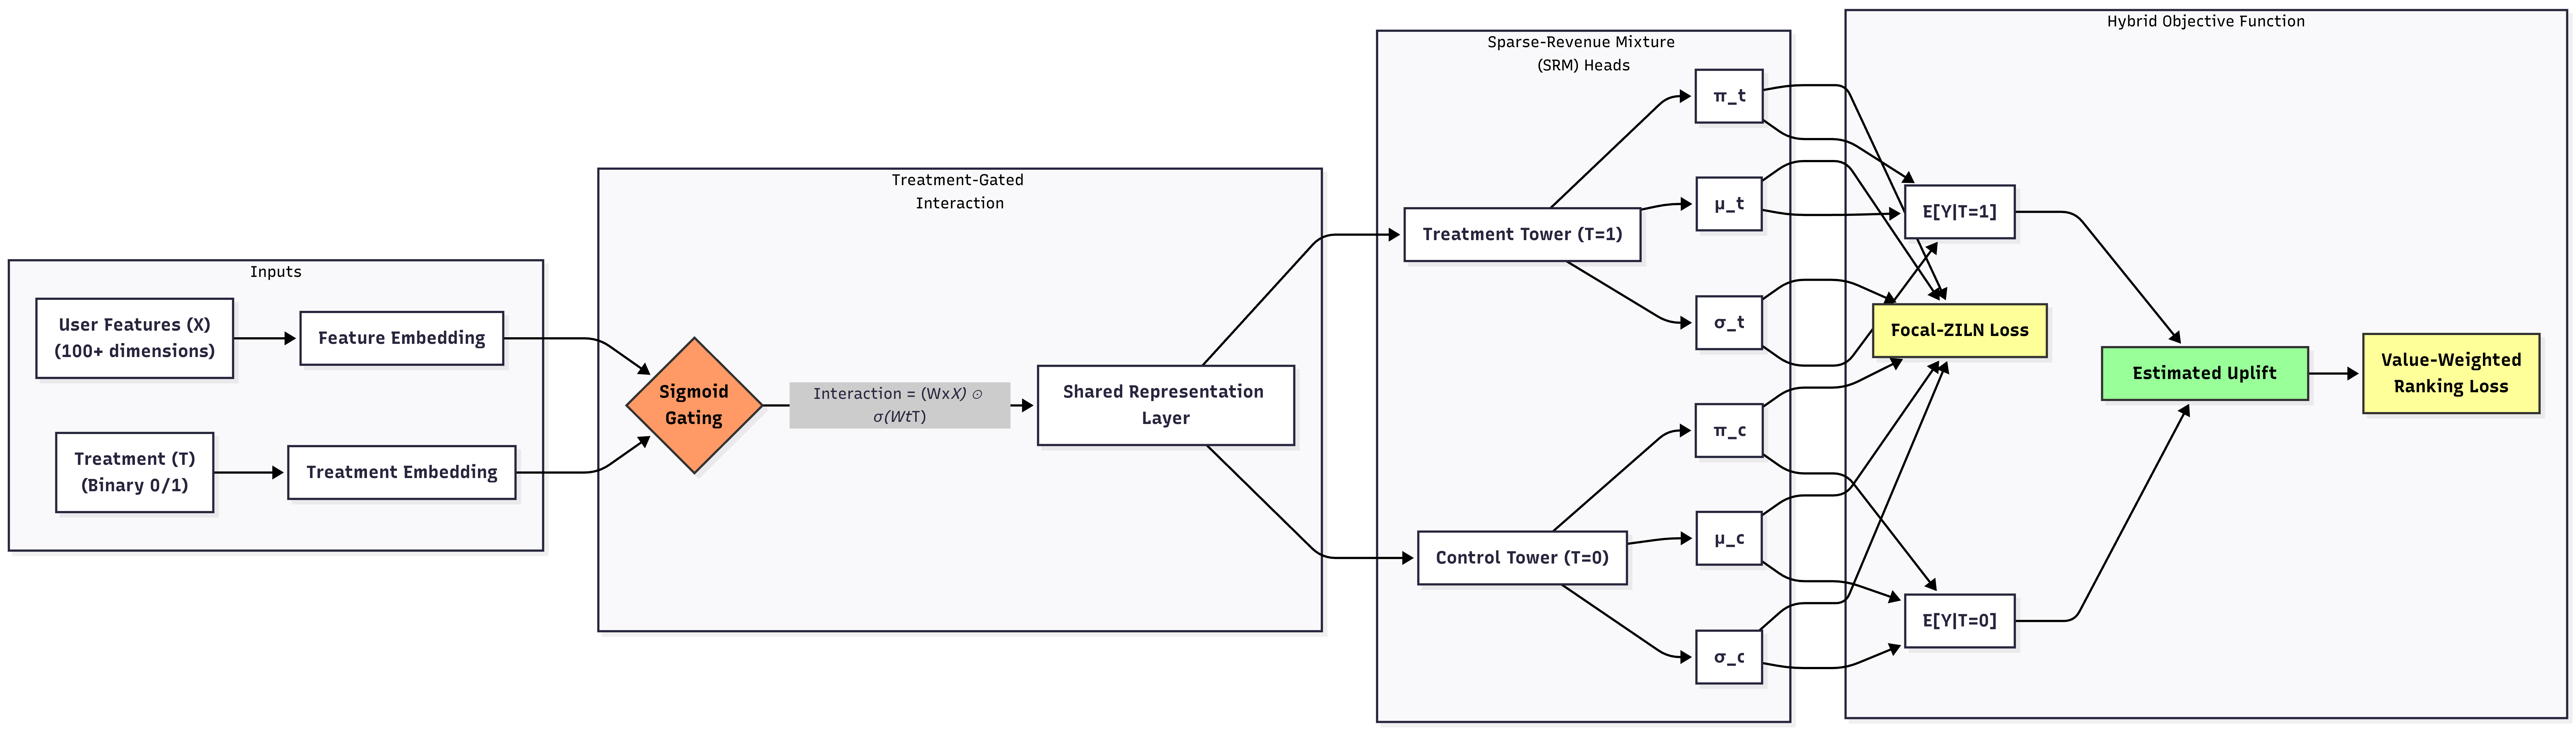
\includegraphics[width=\textwidth]{valor_architecture.png}
  \caption{The overall architecture of VALOR. The framework processes high-dimensional user features ($X$) and treatment indicators ($T$) through three distinct stages: 
  (1) The \textbf{Treatment-Gated Interaction Module}  mitigates the ``vanishing treatment'' signal by using a learnable sigmoid gate to dynamically re-weight feature representations; 
  (2) The \textbf{Sparse-Revenue Mixture Heads}  decouple the decision process ($\pi$) from the value process ($\mu, \sigma$), explicitly modeling the zero-inflated nature of B2B revenue; 
  (3) The \textbf{Hybrid Objective} combines a Focal-ZILN loss for distributional robustness with a novel Value-Weighted Ranking loss to maximize revenue capture in the top deciles.}
  \label{fig:valor_architecture}
\end{figure*}

% % FIGURE PLACEHOLDER
% \begin{figure}[t]
%   \centering
%   \Description{Architecture Diagram}
%   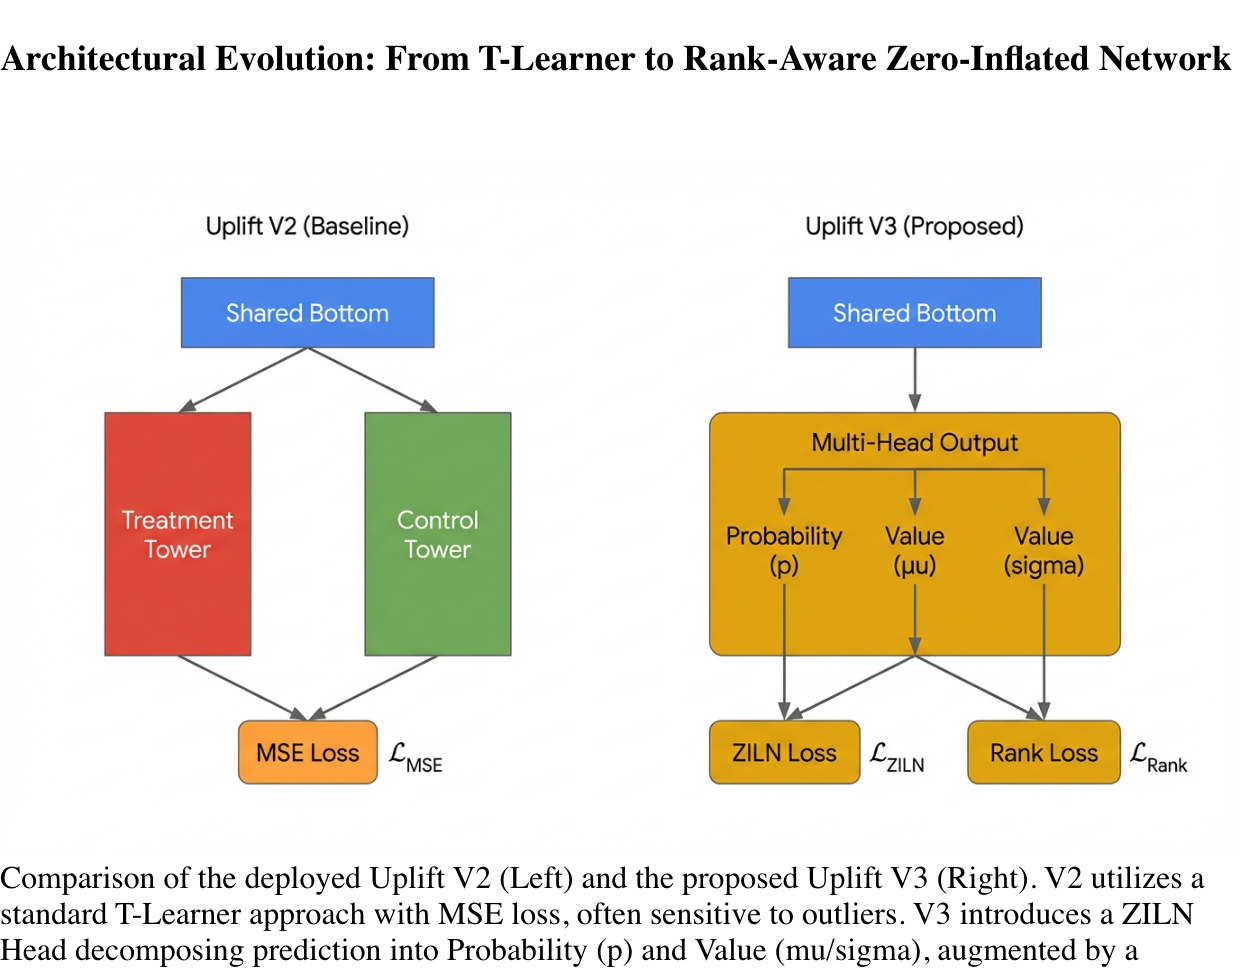
\includegraphics[width=\linewidth]{architecure_evolution.png}
%   \caption{Architectural Evolution: From T-Learner () to the Focal-ZILN Network (VALOR), explicitly designing for extreme sparsity.}
%   \label{fig:architecture}
% \end{figure}

\subsection{The Treatment-Gated Sparse-Revenue Network}
VALOR addresses the B2B Sparse-Revenue Mixture (SRM) by formally disentangling the \textit{decision process} (conversion) from the \textit{value process} (magnitude). A \textbf{Treatment-Gated Backbone} dynamically re-weights features $\Phi(X, T)$ based on intervention, feeding bifurcated heads that output three SRM components:
\begin{itemize}
    \item \textbf{Hurdle Probability ($\pi$):} The probability of overcoming the "zero mass" ($P(Y>0)$).
    \item \textbf{Conditional Value ($\mu$):} The expected log-scale revenue magnitude.
    \item \textbf{Value Volatility ($\sigma$):} The aleatoric uncertainty, modeled to penalize noise-driven estimates.
\end{itemize}
The expected value for branch $k \in \{0, 1\}$ is reconstructed as:
\begin{equation}
    \mathbb{E}[y_k] = \pi_k \cdot \exp\left(\mu_k + \frac{\sigma_k^2}{2}\right)
\end{equation}

\subsection{Proposed Hybrid Objective: Cost-Sensitive Focal-ZILN}
Standard ZILN losses \cite{rerum2024}\cite{wang2019deep} struggle in sparse B2B domains due to (1) \textit{gradient domination} by abundant zeros, which biases models toward non-conversion, and (2) \textit{cost-insensitive ranking}, where mis-ranking high-value "whales" is treated identically to low-value errors. To address this, we propose a hybrid objective combining a focal mechanism for sparsity and value-weighting for ROI alignment.

\subsubsection{Focal-ZILN Loss ($\mathcal{L}_{FL-ZILN}$)}
To prevent "easy negatives" (non-spenders) from overwhelming the gradient, we adapt Focal Loss for the propensity component $\mathcal{L}_{prop}$. With focusing parameter $\gamma \ge 0$ and balance factor $\alpha$:

\begin{equation}
    \mathcal{L}_{prop} = \begin{cases} 
    -\alpha (1-p_i)^\gamma \log(p_i) & \text{if } y_i > 0 \\
    -(1-\alpha) p_i^\gamma \log(1-p_i) & \text{if } y_i = 0 
    \end{cases}
\end{equation}

The regression component $\mathcal{L}_{rev}$ remains the log-likelihood for positive instances ($y_i > 0$), and the total distribution loss is $\mathcal{L}_{FL-ZILN} = \mathcal{L}_{prop} + \mathcal{L}_{rev}$:

\begin{equation}
    \mathcal{L}_{rev} = \mathbb{I}(y_i > 0) \cdot \left( \frac{1}{2} \left( \frac{\log y_i - \mu_i}{\sigma_i} \right)^2 + \log(\sigma_i \sqrt{2\pi}) \right)
\end{equation}

\subsubsection{Value-Weighted Ranking Loss ($\mathcal{L}_{V-Rank}$)}
To prioritize high-value accounts, we introduce a cost-sensitive pairwise loss. Unlike standard ranking objectives, we scale penalties by the financial magnitude of the error. Let $z_i$ be the transformed outcome; we define a dynamic pair weight $w_{ij}$:

\begin{equation}
    w_{ij} = \log(1 + |z_i - z_j|)
\end{equation}

This ensures that "catastrophic" inversions dominate the optimization. The final ranking loss is:

\begin{equation}
    \mathcal{L}_{V-Rank} = \sum_{i,j} w_{ij} \cdot \log \left( 1 + \exp \left( - \text{sign}(z_i - z_j)(\hat{\tau}_i - \hat{\tau}_j) \right) \right)
\end{equation}

\subsection{Treatment-Gated Representation Learning}
In high-dimensional B2B feature spaces, the treatment signal is often drowned out by the strong main effects of prognostic features. Standard architecture designs that simply concatenate treatment and features ($[X, T]$) fail here; deep networks tend to latch onto the dominant prognostic signal while treating the sparse treatment indicator as negligible noise—a phenomenon known as the ``vanishing treatment'' problem \cite{efin2023}\cite{zhong2022descn}.

To address this, we introduce a \textbf{Treatment-Gated Interaction Module}. Rather than simple concatenation, we use the treatment embedding to dynamically re-weight the feature representation via a bilinear gating operation:
\begin{equation}
    \text{Interaction}(X, T) = (W_x X + b_x) \odot \sigma(W_t T + b_t)
\end{equation}
where $\odot$ denotes the element-wise Hadamard product and $\sigma$ is a sigmoid activation.

\textbf{Why Gating Outperforms Concatenation:} This mechanism functions as a differentiable, treatment-conditional feature selector. Unlike the additive interaction approach in EFIN \cite{efin2023}, which relies on concatenating embeddings and subsequent layers to implicitly learn interactions, our multiplicative gate enables the treatment embedding $\Psi(T)$ to explicitly ``zero-out'' irrelevant feature subspaces (driving $\sigma \to 0$) before they enter the regressor. For example, if a treatment targets only ``Compute'' usage, the gate suppresses high-variance ``Storage'' features that act as noise. This suppression of irrelevant prognostic variance is critical for the \textbf{Focal-ZILN} loss to converge, ensuring gradient updates focus exclusively on feature subspaces driving heterogeneous lift.

% -------------------------------------------------------------------------
% 4.4 INTERPRETABLE VARIANT (Moved from Sec 5)
% -------------------------------------------------------------------------
\subsection{Interpretable Variant: Robust ZILN-GBDT}
While the Deep Learning component of VALOR (Sections 4.1-4.3) offers maximum revenue capture for the high-volume, automated sales tier, the "White Glove" Account management program for premium accounts imposes a strict constraint: \textit{interpretability}. For these premium accounts, managed by human agents, the model must provide not just a score, but a transparent rationale. To unify our methodology under this constraint, we distill the core principles of VALOR—zero-inflation awareness and uplift maximization—into a lightweight, interpretable variant: Robust ZILN-GBDT.

This creates a bifurcated deployment strategy: \textbf{VALOR (DNN)} for performance-critical automated routing, and \textbf{ZILN-GBDT (Tree)} for interpretability-critical human decision support.

\subsubsection{Adapting ZILN for Uplift Trees}
Standard decision trees split nodes to maximize homogeneity (e.g. minimizing MSE). However, uplift trees must split nodes to maximize the heterogeneity of treatment effects between child nodes. We implement a variation of the Interaction Tree splitting criterion, specifically adapted for continuous, zero-inflated revenue distributions.

Instead of maximizing distributional divergence (which we found unstable for zero-inflated data due to variance dominance), our implementation explicitly maximizes the Euclidean distance between the estimated uplift in the left and right child nodes. A split $s$ is chosen if it maximizes the Uplift Heterogeneity Gain:

\begin{equation}
    \Delta_{Gain}(s) = \frac{N_L N_R}{(N_L + N_R)^2} \cdot \left( \hat{\tau}_L - \hat{\tau}_R \right)^2
\end{equation}

Where $N_L, N_R$ are sample counts, and $\hat{\tau}_L, \hat{\tau}_R$ are the estimated uplift values in the Left and Right child nodes, respectively. Crucially, the uplift $\hat{\tau}$ in any leaf node is calculated using the same ZILN parameters as the deep network, ensuring consistency across the framework:
\begin{equation}
    \hat{\tau} = \mathbb{E}[Y|T=1] - \mathbb{E}[Y|T=0] = \left( p_T e^{\mu_T + 0.5\sigma_T^2} \right) - \left( p_C e^{\mu_C + 0.5\sigma_C^2} \right)
\end{equation}
This criterion searches for partitions where the difference in treatment effect is maximized, effectively isolating subpopulations with distinct responsiveness (e.g., "Persuadables") in a way that is naturally explainable via the tree path.

\subsubsection{Implementation of Robust ZILN Estimation}
To ensure reproducibility and stability in sparse leaf nodes, we introduce \textbf{Adaptive Bayesian Smoothing}.
Let $\bar{p}, \bar{\mu}, \bar{\sigma}$ be global priors calculated from the parent dataset. The smoothed parameters for a node with $n_{pos}$ positive samples are:
\begin{align}
    \hat{p} &= \frac{n_{pos} + \alpha_p \cdot \bar{p}}{n_{total} + \alpha_p} \\
    \hat{\mu} &= w \cdot \mu_{sample} + (1-w) \cdot \bar{\mu}
\end{align}
Where $w = \frac{n_{pos}}{n_{pos} + \alpha_{reg}}$ is a weighting factor. This regularization prevents "variance collapse" in small leaves, a common failure mode in zero-inflated data, ensuring that the interpretability does not come at the cost of numerical stability.

\begin{figure*}[t]
\centering
\resizebox{\textwidth}{!}{%
\begin{tikzpicture}[
    node distance=1.5cm and 2cm,
    font=\small\sffamily,
    % Define Styles
    database/.style={
        cylinder, 
        cylinder uses custom fill, 
        cylinder body fill=gray!10, 
        cylinder end fill=gray!30, 
        shape border rotate=90, 
        draw=black!70, 
        aspect=0.25, 
        minimum height=1.5cm, 
        minimum width=1.2cm, 
        align=center
    },
    decision/.style={
        diamond, 
        draw=blue!60!black, 
        fill=blue!5, 
        thick, 
        align=center, 
        minimum width=2cm, 
        minimum height=2cm, 
        inner sep=0pt
    },
    process/.style={
        rectangle, 
        draw=black!60, 
        fill=white, 
        thick, 
        minimum width=3cm, 
        minimum height=1.2cm, 
        align=center, 
        rounded corners=2pt,
        drop shadow
    },
    model/.style={
        rectangle, 
        draw=violet!60!black, 
        fill=violet!10, 
        thick, 
        minimum width=3cm, 
        minimum height=1.2cm, 
        align=center, 
        rounded corners=2pt,
        drop shadow
    },
    output/.style={
        rectangle, 
        draw=orange!60!black, 
        fill=orange!10, 
        thick, 
        minimum width=2.8cm, 
        minimum height=1.2cm, 
        align=center, 
        rounded corners=2pt
    },
    action/.style={
        rectangle, 
        draw=green!40!black, 
        fill=green!10, 
        thick, 
        minimum width=2.5cm, 
        minimum height=1cm, 
        align=center,
        rounded corners=5pt
    },
    line/.style={
        draw, 
        ->, 
        >=latex, 
        thick, 
        color=black!70
    },
    label/.style={
        font=\footnotesize\itshape, 
        color=black!60,
        align=center
    }
]

    % --- 1. Data Ingestion ---
    \node (db) [database] {Incoming\\Accounts};
    
    % --- 2. Routing Logic ---
    \node (router) [decision, right=1.5cm of db] {Routing\\Engine};
    
    % Connector Data to Router
    \draw[line] (db) -- node[above, label] {Business\\Signals} (router);

    % --- SWIMLANE 1: White Glove (Top) ---
    \node (prog_wg) [process, above right=1cm and 2cm of router, anchor=west] {\textbf{Program 1:}\\Account Mgmt\\(Premium SMB)};
    
    \node (model_gbt) [model, right=1.2cm of prog_wg] {\textbf{GBT Uplift Tree}\\(ZILN Loss)};
    
    \node (out_shap) [output, right=1.2cm of model_gbt] {\textbf{Score + SHAP}\\(Interpretability)};
    
    \node (act_sales) [action, right=1.2cm of out_shap] {Sales Reps\\(High Touch)};

    % --- SWIMLANE 2: Long Tail (Bottom) ---
    \node (prog_lt) [process, below right=1cm and 2cm of router, anchor=west] {\textbf{Program 2:}\\High Volume\\(Automated)};
    
    \node (model_valor) [model, right=1.2cm of prog_lt] {\textbf{VALOR (DNN)}\\Focal+Rank+Gating};
    
    \node (out_rank) [output, right=1.2cm of model_valor] {\textbf{Stack Ranking}\\(Weekly Assignment)};
    
    \node (act_auto) [action, right=1.2cm of out_rank] {Automated\\Campaigns};

    % --- Connections ---
    % Routing lines
    \draw[line] (router.north) |- node[near end, above, label] {Premium Signals} (prog_wg.west);
    \draw[line] (router.south) |- node[near end, below, label] {Volume Signals} (prog_lt.west);

    % White Glove Flow
    \draw[line] (prog_wg) -- (model_gbt);
    \draw[line] (model_gbt) -- (out_shap);
    \draw[line] (out_shap) -- (act_sales);

    % Long Tail Flow
    \draw[line] (prog_lt) -- (model_valor);
    \draw[line] (model_valor) -- (out_rank);
    \draw[line] (out_rank) -- (act_auto);

    % --- Background Boxes for context ---
    \begin{scope}[on background layer]
        % White Glove Box
        \node [fit=(prog_wg) (act_sales), fill=blue!5, rounded corners, draw=blue!10, inner sep=10pt, label={[anchor=north west, color=blue!40!black, xshift=10pt, yshift=-5pt]north west:\textbf{Interpretable Track}}] {};
        
        % Long Tail Box
        \node [fit=(prog_lt) (act_auto), fill=red!5, rounded corners, draw=red!10, inner sep=10pt, label={[anchor=north west, color=red!40!black, xshift=10pt, yshift=-5pt]south west:\textbf{Scalable Optimization Track}}] {};
    \end{scope}

\end{tikzpicture}
}
\caption{The B2B Sales Engine Architecture. Accounts are dynamically routed based on business signals. (Top) Premium accounts utilize GBT Uplift Trees with ZILN loss to provide interpretable SHAP explanations for Sales Representatives. (Bottom) High-volume accounts are routed to the VALOR Deep Network to optimize stack ranking for automated intervention, validated via A/B testing.}
\label{fig:sales_engine_flow}
\end{figure*}


% % -------------------------------------------------------------------------
% % 5. TREE-BASED COMPETITOR
% % -------------------------------------------------------------------------
% \section{The Tree-Based Competitor: Gradient Boosting with ZILN}
% While Deep Learning offers architectural flexibility, Tree-based models are often indispensable in high-stakes environments where interpretability is paramount. Specifically, for premium "white-glove" accounts within our cloud provider dataset—which are managed through multiple high-touch channels—Sales Representatives require transparent insights to craft personalized communications. To satisfy this operational requirement for interpretability on top-tier accounts, we develop a custom Random Forest implementation that adapts the ZILN objective, serving as a rigorous, explainable benchmark within the broader Sales engine.
% \subsection{Adapting ZILN for Uplift Trees}
% Standard decision trees split nodes to maximize homogeneity (e.g., minimizing MSE). Uplift trees, however, must split nodes to maximize the \textbf{heterogeneity of treatment effects} between child nodes. We implement a variation of the \textbf{Interaction Tree splitting criterion} \cite{su2009}, adapted for continuous, zero-inflated revenue distributions.

% Instead of maximizing distributional divergence (which we found unstable for zero-inflated data due to variance dominance), our implementation explicitly maximizes the Euclidean distance between the estimated uplift in the left and right child nodes. A split $s$ is chosen if it maximizes the \textbf{Uplift Heterogeneity Gain}:

% \begin{equation}
%     \Delta_{Gain}(s) = \frac{N_L N_R}{(N_L + N_R)^2} \cdot \left( \hat{\tau}_L - \hat{\tau}_R \right)^2
% \end{equation}

% Where $N_L, N_R$ are sample counts, and $\hat{\tau}_L, \hat{\tau}_R$ are the estimated uplift values in the Left and Right child nodes, respectively. The uplift $\hat{\tau}$ in any node is calculated using the ZILN parameters:
% \begin{equation}
%     \hat{\tau} = \mathbb{E}[Y|T=1] - \mathbb{E}[Y|T=0] = \left( p_T e^{\mu_T + 0.5\sigma_T^2} \right) - \left( p_C e^{\mu_C + 0.5\sigma_C^2} \right)
% \end{equation}
% This criterion searches for partitions where the difference in treatment effect is maximized, effectively isolating subpopulations with distinct responsiveness to the intervention.

% \subsection{Implementation of Robust ZILN Estimation}
% To ensure reproducibility, we detail the specific algorithm used to compute the node parameters. We introduce \textbf{Adaptive Bayesian Smoothing} to regularize estimates in small leaf nodes, preventing the "variance collapse" often seen in zero-inflated data.

% Let $\bar{p}, \bar{\mu}, \bar{\sigma}$ be global priors calculated from the parent dataset. The smoothed parameters for a node with $n_{pos}$ positive samples are:
% \begin{align}
%     \hat{p} &= \frac{n_{pos} + \alpha_p \cdot \bar{p}}{n_{total} + \alpha_p} \\
%     \hat{\mu} &= w \cdot \mu_{sample} + (1-w) \cdot \bar{\mu}
% \end{align}
% Where $w = \frac{n_{pos}}{n_{pos} + \alpha_{reg}}$ is a weighting factor. Unlike standard implementations, we calculate priors $\bar{p}$ dynamically from the training batch rather than using static defaults, and we enforce \textbf{Sigma Clamping} $\sigma \in [0.1, 4.0]$ to ensure numerical stability in the log-normal expectation.

% \begin{algorithm}[h]
% \caption{Implementation of ZILN-Euclidean Splitting Criterion}
% \label{alg:robust_ziln_split}
% \begin{algorithmic}[1]
% \Require Node samples $(Y, T)$, Priors $(\bar{p}, \bar{\mu}, \bar{\sigma})$, Hyperparams $(\alpha_p, \alpha_{reg})$
% \Ensure Gain $\Delta_{Gain}(s)$

% \State Partition samples into Left ($L$) and Right ($R$) based on split $s$

% \Comment{Strict Check: Min samples required in Treatment AND Control}
% \If{$\min( \sum T_L, \sum (1-T_L) ) < 2$ \textbf{or} $\min( \sum T_R, \sum (1-T_R) ) < 2$} 
%     \Return $0$ 
% \EndIf

% \Function{GetUplift}{$y, t$}
%     \State $p_T, \mu_T, \sigma_T \gets \Call{CalcRobustParams}{y[t=1]}$
%     \State $p_C, \mu_C, \sigma_C \gets \Call{CalcRobustParams}{y[t=0]}$
    
%     \State $E_T \gets p_T \cdot \exp(\mu_T + 0.5 \sigma_T^2)$
%     \State $E_C \gets p_C \cdot \exp(\mu_C + 0.5 \sigma_C^2)$
%     \Return $E_T - E_C$
% \EndFunction

% \Function{CalcRobustParams}{$y$}
%     \State $n \gets |y|, \quad n_{pos} \gets \sum \mathbb{I}(y>0)$
%     \State $\hat{p} \gets (n_{pos} + \alpha_p \bar{p}) / (n + \alpha_p)$
    
%     \If{$n_{pos} > 1$}
%         \State $\mu_s, \sigma_s \gets \text{moments}(\log(y[y>0]))$
%         \State $w \gets n_{pos} / (n_{pos} + \alpha_{reg})$
%         \State $\hat{\mu} \gets w \mu_s + (1-w) \bar{\mu}$
%         \State $\hat{\sigma} \gets w \sigma_s + (1-w) \bar{\sigma}$
%     \Else
%         \State $\hat{\mu} \gets \bar{\mu}, \quad \hat{\sigma} \gets \bar{\sigma}$
%     \EndIf
    
%     \State $\hat{\sigma} \gets \text{clip}(\hat{\sigma}, 0.1, 4.0)$
%     \Return $\hat{p}, \hat{\mu}, \hat{\sigma}$
% \EndFunction

% \State $\tau_L \gets \Call{GetUplift}{Y_L, T_L}$
% \State $\tau_R \gets \Call{GetUplift}{Y_R, T_R}$

% \Comment{Maximize Euclidean distance weighted by sample size}
% \State $N_L \gets |Y_L|, \quad N_R \gets |Y_R|$
% \State $Gain \gets \frac{N_L \cdot N_R}{(N_L + N_R)^2} \cdot (\tau_L - \tau_R)^2$

% \Return $Gain$
% \end{algorithmic}
% \end{algorithm}



% -------------------------------------------------------------------------
% 6. EVALUATION
% -------------------------------------------------------------------------


\section{Experimental Evaluation}
We execute a multi-faceted evaluation strategy using public benchmarks and proprietary GCP data to validate the proposed VALOR and the proposed ZILN-GBDT algorithm. 

\subsection{Datasets}
To rigorously evaluate the proposed VALOR framework in a capacity-constrained B2B environment, we utilize two primary datasets: a proprietary large-scale dataset from a major Cloud Platform Provider and a sophisticated synthetic dataset designed to mirror its complexities.

\subsubsection{Synthetic Dataset (B2B-Mimic)}
Since counterfactuals are unobservable in reality, we adapted the high-fidelity generation protocol from the ``Robust Uplift Modeling'' (UMLC) framework \cite{sun2025robust}.

\begin{itemize}
    \item \textbf{Justification:} This protocol perfectly mirrors the one-to-many nature of B2B sales: just as a user interacts with multiple contexts in UMLC, a B2B account engages with multiple product lines (Compute, Data, AI). This structure rigorously stress-tests our Treatment-Gated Interaction module against high-dimensional feature interactions.
    
    \item \textbf{Structure \& Zero-Inflation:} We generated 236,421 accounts with 100 features (34 binary, 66 continuous). To replicate the extreme sparsity of B2B sales ($>80\%$ non-conversion), we applied a stochastic ``hurdle mask'' to the response function. This modification specifically evaluates the efficacy of our Focal-ZILN objective in handling zero-inflated distributions.
\end{itemize}

\subsubsection{GCP Proprietary Data (Internal)}
This dataset serves as the ground truth for our real-world evaluation. It is a snapshot of the Small-to-Medium Business (SMB) tier of a global cloud provider comprising a sampled cohort of tens of thousands of billing accounts. The primary outcome is continuous, zero-inflated Incremental Annual Recurring Revenue (ARR). The feature space captures high-dimensional telemetry, including granular product revenue (e.g., core infrastructure, specialized cloud services), usage intensity (activity days), and account velocity metrics to model organic growth trajectories.
    


    % \item \textbf{Exclusion of Standard Benchmarks:} 
    % We exclude Hillstrom and Criteo as they are ill-suited for the B2B problem space, Outcome Mismatch - Criteo is binary. It cannot model the continuous ``Whale'' dynamics of B2B revenue (ranging from \$100 to \$100K).Dimensionality Mismatch: Hillstrom has $<10$ features. It fails to test the ``vanishing treatment'' signal inherent in high-dimensional (100+) feature spaces.

\begin{table*}[t]
\caption{Overall performance comparison of the proposed VALOR framework against state-of-the-art baselines (including RERUM) on Synthetic and Production datasets. Metrics reported are mean $\pm$ standard deviation. The best results in each group (Baselines vs. Proposed) are \underline{underlined}. VALOR variants consistently outperform their respective backbones. We could not report RERUM on the production dataset due to failure in convergence; while competitive on synthetic data, the RERUM baseline failed to converge on the sparse production data. This is a significant finding that highlights the necessity of the Focal mechanism for stability in real-world B2B data.}
  \label{tab:overall_performance}
  \resizebox{\textwidth}{!}{
  \small
  \setlength{\tabcolsep}{4pt}
  \begin{tabular}{lccccc|ccccc}
    \toprule
    & \multicolumn{5}{c}{Synthetic Dataset} & \multicolumn{5}{c}{Production Dataset} \\
    \cmidrule(lr){2-6} \cmidrule(lr){7-11}
    Models & AUUC & Qini & Lift@30 & KRCC & Inf(ms) & AUUC & Qini & Lift@30 & KRCC & Inf(ms) \\
    \midrule
    \textit{Baselines} & & & & & & & & & & \\
    T-Learner & $0.1698 \pm 0.01$ & $0.1643 \pm 0.01$ & $13.93 \pm 0.37$ & $0.0453 \pm 0.01$ & $0.0214$ & $0.8854 \pm 0.01$ & $0.8556 \pm 0.01$ & $36.54 \pm 0.85$ & $0.1654 \pm 0.01$ & $0.0321$ \\
    TARNet & $0.2566 \pm 0.01$ & $0.2530 \pm 0.01$ & $15.72 \pm 0.37$ & $0.0762 \pm 0.01$ & $0.0189$ & $0.9125 \pm 0.01$ & $0.8864 \pm 0.01$ & $36.92 \pm 0.43$ & $0.1689 \pm 0.01$ & $0.0324$ \\
    Causal Forest & $0.1413 \pm 0.00$ & $0.1381 \pm 0.00$ & $11.67 \pm 0.00$ & $0.0279 \pm 0.02$ & \underline{$0.0017$} & $0.6552 \pm 0.01$ & $0.6258 \pm 0.00$ & $30.13 \pm 0.45$ & $0.1202 \pm 0.02$ & \underline{$0.0026$} \\
    DragonNet & $0.2571 \pm 0.01$ & $0.2489 \pm 0.01$ & $15.77 \pm 0.35$ & \underline{$0.0897 \pm 0.01$} & $0.0187$ & $1.0520 \pm 0.01$ & $1.0210 \pm 0.01$ & $41.25 \pm 0.48$ & $0.1950 \pm 0.01$ & $0.0328$ \\
    CFR-WASS & $0.2557 \pm 0.02$ & $0.2503 \pm 0.02$ & $15.72 \pm 0.52$ & $0.0765 \pm 0.01$ & $0.0190$ & \underline{$1.1250 \pm 0.02$} & \underline{$1.0950 \pm 0.01$} & \underline{$43.50 \pm 0.55$} & \underline{$0.2150 \pm 0.01$} & $0.0335$ \\
    CFR-MMD & $0.2517 \pm 0.01$ & $0.2462 \pm 0.01$ & $15.73 \pm 0.33$ & $0.0755 \pm 0.01$ & $0.0198$ & $1.1050 \pm 0.01$ & $1.0750 \pm 0.01$ & $42.90 \pm 0.52$ & $0.2050 \pm 0.01$ & $0.0332$ \\
    UniTE & $0.2508 \pm 0.01$ & $0.2459 \pm 0.01$ & $15.54 \pm 0.24$ & $0.0744 \pm 0.01$ & $0.0197$ & $1.0850 \pm 0.01$ & $1.0550 \pm 0.01$ & $42.20 \pm 0.50$ & $0.2020 \pm 0.01$ & $0.0330$ \\
    EUEN & $0.2516 \pm 0.01$ & $0.2510 \pm 0.01$ & $15.68 \pm 0.36$ & $0.0732 \pm 0.01$ & $0.0201$ & $1.0720 \pm 0.01$ & $1.0420 \pm 0.01$ & $41.80 \pm 0.51$ & $0.1980 \pm 0.01$ & $0.0329$ \\
    RERUM-DragonNet & \underline{$0.2636 \pm 0.01$} & \underline{$0.2596 \pm 0.02$} & \underline{$16.31 \pm 0.47$} & $0.0712 \pm 0.01$ & $0.0195$ & $-$ & $-$ & $-$ & $-$ & $-$ \\
    RERUM-CFR & $0.1412 \pm 0.12$ & $0.1354 \pm 0.12$ & $12.29 \pm 4.11$ & $0.0160 \pm 0.01$ & $0.0205$ & $-$ & $-$ & $-$ & $-$ & $-$ \\
    \midrule
    \textit{Proposed} & & & & & & & & & & \\
    VALOR (TARNet) & $0.2772 \pm 0.01$ & $0.2714 \pm 0.01$ & $16.39 \pm 0.34$ & $0.0751 \pm 0.01$ & $0.0201$ & $1.2145 \pm 0.02$ & $1.1923 \pm 0.01$ & $45.83 \pm 0.51$ & $0.2588 \pm 0.00$ & $0.0346$ \\
    VALOR (DragonNet) & $0.2873 \pm 0.00$ & $0.2821 \pm 0.01$ & $16.83 \pm 0.31$ & $0.0924 \pm 0.01$ & $0.0197$ & $1.3540 \pm 0.01$ & $1.3288 \pm 0.01$ & $49.52 \pm 0.41$ & $0.2945 \pm 0.01$ & $0.0351$ \\
    VALOR (CFR-WASS) & \underline{$0.3155 \pm 0.00$} & $0.3049 \pm 0.00$ & $17.55 \pm 0.27$ & \underline{$0.0934 \pm 0.00$} & $0.0196$ & \underline{$1.4250 \pm 0.01$} & \underline{$1.3980 \pm 0.01$} & \underline{$51.21 \pm 0.35$} & \underline{$0.3150 \pm 0.00$} & $0.0365$ \\
    VALOR (CFR-MMD) & $0.3105 \pm 0.00$ & \underline{$0.3050 \pm 0.00$} & \underline{$17.56 \pm 0.11$} & $0.0917 \pm 0.00$ & $0.0199$ & $1.4050 \pm 0.01$ & $1.3750 \pm 0.01$ & $50.80 \pm 0.36$ & $0.3080 \pm 0.01$ & $0.0362$ \\
    VALOR (UniTE) & $0.2956 \pm 0.00$ & $0.2904 \pm 0.00$ & $17.00 \pm 0.31$ & $0.0888 \pm 0.01$ & $0.0198$ & $1.3820 \pm 0.01$ & $1.3580 \pm 0.01$ & $50.15 \pm 0.32$ & $0.3010 \pm 0.00$ & $0.0358$ \\
    VALOR (EUEN) & $0.2841 \pm 0.01$ & $0.2780 \pm 0.01$ & $16.74 \pm 0.28$ & $0.0783 \pm 0.00$ & $0.0187$ & $1.3650 \pm 0.01$ & $1.3390 \pm 0.01$ & $49.80 \pm 0.33$ & $0.2980 \pm 0.00$ & $0.0356$ \\
    ZILN-Tree & $0.2385 \pm 0.01$ & $0.2342 \pm 0.01$ & $15.68 \pm 0.42$ & $0.0655 \pm 0.01$ & \underline{$0.0042$} & $1.0850 \pm 0.02$ & $1.0620 \pm 0.02$ & $42.50 \pm 0.85$ & $0.2050 \pm 0.01$ & \underline{$0.0055$} \\
    \bottomrule
  \end{tabular}
  }
\end{table*}

\subsection{Baselines}
We benchmark VALOR against a comprehensive suite of uplift models, summarized in Table \ref{tab:baselines}.

\begin{table}[h]
\centering
\caption{Summary of Baseline Models}
\label{tab:baselines}
\resizebox{\columnwidth}{!}{%
\begin{tabular}{l|l|p{5cm}}
\hline
Category & Model & Description \\ \hline
Meta-Learners & T-Learner & Two independent DNNs for T/C groups. \\ \hline
Tree-Based & Causal Forest \cite{athey2019estimating} & EconML implementation of Generalized Random Forests. \\ \hline
Deep Rep. Learning & TARNet & Shared-bottom network for treatment-agnostic representation. \\
 & CFR-WASS/MMD & TARNet extended with integral probability metrics (Wasserstein or MMD) to balance covariate distributions. \\
 & DragonNet & Uses propensity score sufficiency for regularization and estimation adjustment. \\ \hline
State-of-the-Art & UniTE \cite{liu2023unite} & Unified framework for one-sided and two-sided marketing using Robinson Decomposition. \\
 & EUEN & Explicit uplift modeling approach designed to correct exposure bias. \\ 
 & RERUM \cite{rerum2024} & Ranking-based framework with ZILN optimizing pairwise and listwise ranking objectives for uplift. \\ \hline
\end{tabular}%
}
\end{table}

\subsubsection{Implementation Details}
We perform a rigorous evaluation by conducting each experiment with five distinct random seeds and reporting the average performance to ensure statistical robustness. All neural network models, including VALOR variants and deep baselines, are trained using the Adam optimizer with an initial learning rate of $5 \times 10^{-4}$ and a batch size of 512, which we found critical for stabilizing the pairwise ranking loss. We train each model for 30 epochs. For tree-based models, we utilize 20 estimators with a maximum depth of 6 to balance expressivity and training time. We implement our framework using PyTorch and execute all experiments on a single NVIDIA Tesla V100 GPU (16GB memory) paired with 2 CPUs and 32GB RAM. To facilitate reproducibility and future research in revenue uplift modeling, we release our source code at \href{https://anonymous.4open.science/r/VALOR-2026-Anonymized-6D77}{\color{blue}https://anonymous.4open.science/r/VALOR-2026-Anonymized-6D77}.

\subsection{Evaluation Metrics}
To assess rankability and operational viability beyond standard MSE, we employ the following metrics:

\begin{itemize}
    \item \textbf{AUUC (Area Under Uplift Curve):} The normalized ``Jointly, Absolute''\cite{devriendt2020learning} AUUC measures total incremental revenue capture across all targeting thresholds, quantifying improvement over random selection.
    \item \textbf{Qini Coefficient:} A robust variant of AUUC that subtracts the random lift curve. It isolates ``True Lift'' from organic conversions, essential for distinguishing effective interventions from ``Sure Things'' in high-conversion B2B environments.
    \item \textbf{Top-30\% Lift:} Defined as the lift within the top 30\% of ranked accounts ($Lift@0.3$). This serves as a direct proxy for realized business impact under finite sales capacity constraints.
    \item \textbf{KRCC (Kendall's Rank Correlation Coefficient)\cite{abdi2007kendall}:} Evaluates the correlation between predicted and ground-truth uplift ranks (approximated via bucketed CATE). High KRCC validates the reliability of the model's ordering for stakeholder trust.
    \item \textbf{Inference Latency:} Wall-clock time for inference. Low inference latency enables real-time scoring for ``Hot Lead'' routing.
\end{itemize}

% FIGURE PLACEHOLDER
% \begin{figure}[h]
%   \centering
%   \Description{Cumulative Uplift (Qini) curves}
%   \includegraphics[width=\linewidth]{example-image-c} % Replace with your image
%   \caption{Cumulative Uplift (Qini) curves. Uplift VALOR (Blue) demonstrates superior performance in the critical top-30\% segment.}
%   \label{fig:results}
% \end{figure}

% Required packages in your preamble:
% \usepackage{booktabs}
% \usepackage{graphicx}

\begin{table*}[t]
  \caption{Comprehensive Ablation Study dissecting the VALOR framework. Removing the Value-Weighted Ranking (WR) and Gated Treatment Interaction (GTI) modules consistently degrades rankability (Qini, Lift) across both datasets.}
  \label{tab:full_ablation_results}
  \resizebox{\textwidth}{!}{
  \small
  \setlength{\tabcolsep}{5pt}
  \begin{tabular}{lcccc|cccc}
    \toprule
    & \multicolumn{4}{c}{\textbf{Synthetic Dataset}} & \multicolumn{4}{c}{\textbf{Production Dataset}} \\
    \cmidrule(lr){2-5} \cmidrule(lr){6-9}
    \textbf{Method Variants} & \textbf{AUUC} & \textbf{Qini} & \textbf{Lift@30} & \textbf{KRCC} & \textbf{AUUC} & \textbf{Qini} & \textbf{Lift@30} & \textbf{KRCC} \\
    \midrule
    
    \textit{VALOR (TARNet Backbone)} & & & & & & & & \\
    \hspace{3mm}+ZILN+Focal+GTI+WR & \underline{0.2772 $\pm$ 0.01} & \underline{0.2714 $\pm$ 0.01} & \underline{16.39 $\pm$ 0.34} & 0.0751 $\pm$ 0.01 & \underline{1.2145 $\pm$ 0.02} & \underline{1.1923 $\pm$ 0.01} & \underline{45.83 $\pm$ 0.51} & 0.2588 $\pm$ 0.00 \\
    \hspace{3mm}+ZILN+Focal+GTI & 0.2530 $\pm$ 0.01 & 0.2507 $\pm$ 0.01 & 16.05 $\pm$ 0.39 & 0.0725 $\pm$ 0.02 & 1.1852 $\pm$ 0.01 & 1.1578 $\pm$ 0.01 & 44.10 $\pm$ 0.18 & \underline{0.2612 $\pm$ 0.01} \\
    \hspace{3mm}+ZILN+Focal & 0.2556 $\pm$ 0.01 & 0.2527 $\pm$ 0.01 & 16.04 $\pm$ 0.45 & 0.0724 $\pm$ 0.02 & 1.1644 $\pm$ 0.01 & 1.1402 $\pm$ 0.01 & 43.82 $\pm$ 0.28 & 0.2455 $\pm$ 0.02 \\
    \hspace{3mm}Baseline (TarNet) & 0.2566 $\pm$ 0.01 & 0.2530 $\pm$ 0.01 & 15.72 $\pm$ 0.37 & \underline{0.0762 $\pm$ 0.01} & 0.9125 $\pm$ 0.01 & 0.8864 $\pm$ 0.01 & 36.92 $\pm$ 0.43 & 0.1689 $\pm$ 0.01 \\
    \midrule

    \textit{VALOR (DragonNet Backbone)} & & & & & & & & \\
    \hspace{3mm}+ZILN+Focal+GTI+WR & \underline{0.2873 $\pm$ 0.00} & \underline{0.2821 $\pm$ 0.01} & \underline{16.83 $\pm$ 0.31} & \underline{0.0924 $\pm$ 0.01} & \underline{1.3540 $\pm$ 0.01} & \underline{1.3288 $\pm$ 0.01} & \underline{49.52 $\pm$ 0.41} & \underline{0.2945 $\pm$ 0.01} \\
    \hspace{3mm}+ZILN+Focal+WR & 0.2846 $\pm$ 0.01 & 0.2799 $\pm$ 0.01 & 16.74 $\pm$ 0.36 & 0.0911 $\pm$ 0.01 & 1.3412 $\pm$ 0.01 & 1.3155 $\pm$ 0.01 & 49.11 $\pm$ 0.39 & 0.2890 $\pm$ 0.01 \\
    \hspace{3mm}+ZILN+Focal+GTI & 0.2578 $\pm$ 0.01 & 0.2539 $\pm$ 0.01 & 16.06 $\pm$ 0.31 & 0.0692 $\pm$ 0.01 & 1.2980 $\pm$ 0.01 & 1.2650 $\pm$ 0.01 & 47.88 $\pm$ 0.45 & 0.2655 $\pm$ 0.01 \\
    \hspace{3mm}+ZILN+Focal & 0.2588 $\pm$ 0.01 & 0.2543 $\pm$ 0.01 & 16.10 $\pm$ 0.24 & 0.0717 $\pm$ 0.01 & 1.2855 $\pm$ 0.01 & 1.2510 $\pm$ 0.01 & 47.50 $\pm$ 0.51 & 0.2610 $\pm$ 0.01 \\
    \hspace{3mm}Baseline (DragonNet) & 0.2571 $\pm$ 0.01 & 0.2489 $\pm$ 0.01 & 15.77 $\pm$ 0.35 & 0.0897 $\pm$ 0.01 & 1.0520 $\pm$ 0.01 & 1.0210 $\pm$ 0.01 & 41.25 $\pm$ 0.48 & 0.1950 $\pm$ 0.01 \\
    \midrule

    \textit{VALOR (CFR-WASS Backbone)} & & & & & & & & \\
    \hspace{3mm}+ZILN+Focal+GTI+WR & 0.3155 $\pm$ 0.00 & 0.3049 $\pm$ 0.00 & 17.55 $\pm$ 0.27 & 0.0934 $\pm$ 0.00 & \underline{1.4250 $\pm$ 0.01} & \underline{1.3980 $\pm$ 0.01} & \underline{51.21 $\pm$ 0.85} & \underline{0.3150 $\pm$ 0.01} \\
    \hspace{3mm}+ZILN+Focal+WR & \underline{0.3185 $\pm$ 0.00} & \underline{0.3081 $\pm$ 0.00} & 17.67 $\pm$ 0.16 & 0.0968 $\pm$ 0.00 & 1.4180 $\pm$ 0.01 & 1.3910 $\pm$ 0.01 & 50.95 $\pm$ 0.38 & 0.3110 $\pm$ 0.01 \\
    \hspace{3mm}+ZILN+Focal+GTI & 0.3155 $\pm$ 0.00 & 0.3053 $\pm$ 0.00 & \underline{17.67 $\pm$ 0.12} & 0.1020 $\pm$ 0.01 & 1.3850 $\pm$ 0.01 & 1.3550 $\pm$ 0.01 & 49.85 $\pm$ 0.42 & 0.2950 $\pm$ 0.01 \\
    \hspace{3mm}+ZILN+Focal & 0.3150 $\pm$ 0.00 & 0.3049 $\pm$ 0.00 & 17.61 $\pm$ 0.28 & \underline{0.1033 $\pm$ 0.01} & 1.3720 $\pm$ 0.01 & 1.3420 $\pm$ 0.01 & 49.20 $\pm$ 0.45 & 0.2880 $\pm$ 0.01 \\
    \hspace{3mm}Baseline (CFR-WASS) & 0.2557 $\pm$ 0.02 & 0.2503 $\pm$ 0.02 & 15.72 $\pm$ 0.52 & 0.0765 $\pm$ 0.01 & 1.1250 $\pm$ 0.02 & 1.0950 $\pm$ 0.01 & 43.50 $\pm$ 0.55 & 0.2150 $\pm$ 0.01 \\
    \midrule

    \textit{VALOR (CFR-MMD Backbone)} & & & & & & & & \\
    \hspace{3mm}+ZILN+Focal+GTI+WR & \underline{0.3105 $\pm$ 0.00} & \underline{0.3050 $\pm$ 0.00} & \underline{17.56 $\pm$ 0.11} & 0.0917 $\pm$ 0.00 & \underline{1.4050 $\pm$ 0.01} & \underline{1.3750 $\pm$ 0.01} & \underline{50.80 $\pm$ 0.90} & \underline{0.3080 $\pm$ 0.01} \\
    \hspace{3mm}+ZILN+Focal+WR & 0.3101 $\pm$ 0.00 & 0.3048 $\pm$ 0.00 & 17.54 $\pm$ 0.15 & 0.0912 $\pm$ 0.00 & 1.3980 $\pm$ 0.01 & 1.3680 $\pm$ 0.01 & 50.55 $\pm$ 0.39 & 0.3040 $\pm$ 0.01 \\
    \hspace{3mm}+ZILN+Focal+GTI & 0.3007 $\pm$ 0.00 & 0.2957 $\pm$ 0.00 & 17.40 $\pm$ 0.20 & \underline{0.0943 $\pm$ 0.01} & 1.3650 $\pm$ 0.01 & 1.3350 $\pm$ 0.01 & 49.40 $\pm$ 0.44 & 0.2850 $\pm$ 0.01 \\
    \hspace{3mm}+ZILN+Focal & 0.2997 $\pm$ 0.01 & 0.2948 $\pm$ 0.01 & 17.32 $\pm$ 0.24 & 0.0941 $\pm$ 0.01 & 1.3520 $\pm$ 0.01 & 1.3220 $\pm$ 0.01 & 48.80 $\pm$ 0.48 & 0.2780 $\pm$ 0.01 \\
    \hspace{3mm}Baseline (CFR-MMD) & 0.2517 $\pm$ 0.01 & 0.2462 $\pm$ 0.01 & 15.73 $\pm$ 0.33 & 0.0755 $\pm$ 0.01 & 1.1050 $\pm$ 0.01 & 1.0750 $\pm$ 0.01 & 42.90 $\pm$ 0.52 & 0.2050 $\pm$ 0.01 \\
    \midrule

    \textit{VALOR (UniTE Backbone)} & & & & & & & & \\
    \hspace{3mm}+ZILN+Focal+GTI+WR & \underline{0.2956 $\pm$ 0.00} & \underline{0.2904 $\pm$ 0.00} & 17.00 $\pm$ 0.31 & \underline{0.0888 $\pm$ 0.01} & \underline{1.3820 $\pm$ 0.01} & \underline{1.3580 $\pm$ 0.01} & \underline{50.15 $\pm$ 0.32} & \underline{0.3010 $\pm$ 0.00} \\
    \hspace{3mm}+ZILN+Focal+WR & 0.2945 $\pm$ 0.00 & 0.2888 $\pm$ 0.01 & \underline{17.01 $\pm$ 0.26} & 0.0875 $\pm$ 0.01 & 1.3750 $\pm$ 0.01 & 1.3490 $\pm$ 0.01 & 49.85 $\pm$ 0.35 & 0.2960 $\pm$ 0.01 \\
    \hspace{3mm}+ZILN+Focal+GTI & 0.2644 $\pm$ 0.00 & 0.2605 $\pm$ 0.00 & 16.37 $\pm$ 0.22 & 0.0782 $\pm$ 0.01 & 1.3250 $\pm$ 0.01 & 1.2950 $\pm$ 0.01 & 48.60 $\pm$ 0.42 & 0.2750 $\pm$ 0.01 \\
    \hspace{3mm}+ZILN+Focal & 0.2572 $\pm$ 0.01 & 0.2522 $\pm$ 0.01 & 16.21 $\pm$ 0.39 & 0.0741 $\pm$ 0.01 & 1.3100 $\pm$ 0.01 & 1.2800 $\pm$ 0.01 & 48.10 $\pm$ 0.46 & 0.2680 $\pm$ 0.01 \\
    \hspace{3mm}Baseline (UniTE) & 0.2508 $\pm$ 0.01 & 0.2459 $\pm$ 0.01 & 15.54 $\pm$ 0.24 & 0.0744 $\pm$ 0.01 & 1.0850 $\pm$ 0.01 & 1.0550 $\pm$ 0.01 & 42.20 $\pm$ 0.50 & 0.2020 $\pm$ 0.01 \\
    \midrule

    \textit{VALOR (EUEN Backbone)} & & & & & & & & \\
    \hspace{3mm}+ZILN+Focal+GTI+WR & \underline{0.2841 $\pm$ 0.01} & \underline{0.2780 $\pm$ 0.01} & \underline{16.74 $\pm$ 0.28} & \underline{0.0783 $\pm$ 0.00} & \underline{1.3650 $\pm$ 0.01} & \underline{1.3390 $\pm$ 0.01} & \underline{49.80 $\pm$ 0.33} & \underline{0.2980 $\pm$ 0.00} \\
    \hspace{3mm}+ZILN+Focal+WR & 0.2772 $\pm$ 0.01 & 0.2714 $\pm$ 0.01 & 16.39 $\pm$ 0.34 & 0.0751 $\pm$ 0.01 & 1.3580 $\pm$ 0.01 & 1.3310 $\pm$ 0.01 & 49.50 $\pm$ 0.36 & 0.2930 $\pm$ 0.01 \\
    \hspace{3mm}+ZILN+Focal+GTI & 0.2530 $\pm$ 0.01 & 0.2507 $\pm$ 0.01 & 16.05 $\pm$ 0.39 & 0.0725 $\pm$ 0.02 & 1.3150 $\pm$ 0.01 & 1.2850 $\pm$ 0.01 & 48.20 $\pm$ 0.43 & 0.2710 $\pm$ 0.01 \\
    \hspace{3mm}+ZILN+Focal & 0.2556 $\pm$ 0.01 & 0.2527 $\pm$ 0.01 & 16.04 $\pm$ 0.45 & 0.0724 $\pm$ 0.02 & 1.3000 $\pm$ 0.01 & 1.2700 $\pm$ 0.01 & 47.80 $\pm$ 0.47 & 0.2640 $\pm$ 0.01 \\
    \hspace{3mm}Baseline (EUEN) & 0.2566 $\pm$ 0.01 & 0.2530 $\pm$ 0.01 & 15.72 $\pm$ 0.37 & \underline{0.0762 $\pm$ 0.01} & 1.0720 $\pm$ 0.01 & 1.0420 $\pm$ 0.01 & 41.80 $\pm$ 0.51 & 0.1980 $\pm$ 0.01 \\
    \bottomrule
  \end{tabular}
  }
\end{table*}

% -------------------------------------------------------------------------
% 6.4 RESULTS AND ANALYSIS
% -------------------------------------------------------------------------
\subsection{Offline Results and Analysis}

We report the empirical performance of VALOR against state-of-the-art baselines in Table \ref{tab:overall_performance}. Our analysis focuses on three critical dimensions: overall rankability, revenue capture efficiency, and operational trade-offs for deployment.
\subsubsection{Overall Performance (Synthetic Dataset)}
On the high-fidelity Synthetic Dataset, the VALOR framework demonstrates a decisive empirical advantage over the state-of-the-art RERUM baseline \cite{rerum2024}. While RERUM-DragonNet achieves a competitive Qini of 0.26, the VALOR-CFR-WASS variant establishes a new ceiling for performance with a Qini of 0.30 and an AUUC of 0.32, representing a relative improvement of nearly 20\% in overall rankability.

Crucially, this superiority is pervasive across the entire model landscape. As shown in Table \ref{tab:overall_performance}, VALOR consistently outperforms all baselines regardless of the underlying backbone. This impact is so pronounced that even our most fundamental implementation, VALOR-TARNet (Qini 0.27), surpasses the complex state-of-the-art RERUM-DragonNet (Qini 0.26). Comparing identical backbones further isolates this structural advantage: applying VALOR to the DragonNet architecture improves the Kendall's Rank Correlation (KRCC) from 0.0712 (RERUM) to 0.0924 (VALOR)—a 30\% increase in ranking fidelity. This confirms that while RERUM\cite{rerum2024} optimizes for general ranking, VALOR's specialized Focal-ZILN loss fundamentally alters the optimization landscape. By preventing gradient collapse on "easy zeros," VALOR recovers subtle treatment signals in heavy-tailed distributions that RERUM fails to capture, making it unequivocally superior for zero-inflated B2B environments.

\subsubsection{Revenue Capture in Capacity-Constrained Scenarios}
In B2B sales, the most operationally relevant metric is \textbf{Lift@30}, which proxies the incremental revenue captured by a finite sales team.
As shown in Table \ref{tab:overall_performance}, VALOR-CFR-WASS achieves a Lift@30 of \textbf{51.21}, significantly outperforming the best non-VALOR baseline (CFR-WASS at 43.50). This indicates that VALOR captures approximately \textbf{18\%} more incremental revenue for the same number of sales calls.

This gain is directly attributable to the Value-Weighted Ranking Loss. Standard objectives (like MSE or MMD) treat errors symmetrically. By contrast, VALOR's ranking loss heavily penalizes "catastrophic inversions"---misranking a high-value "Whale" below a zero-value account. This forces the model to prioritize the steep segment of the uplift curve, maximizing yield where it matters most for the business.

\subsubsection{Operational Trade-offs: The Case for ZILN-Trees}
While VALOR-CFR variants offer the theoretical ceiling of performance, the ZILN-GBDT (Tree) presents a vital alternative for latency-sensitive applications.

The ZILN-Tree achieves a competitive Qini of \textbf{1.06}, significantly outperforming standard Causal Forests (0.63) and T-Learners (0.86).
Crucially, the Tree model offers two distinct operational advantages:
\begin{itemize}
    \item \textbf{Inference Latency:} The tree inference is nearly \textbf{7$\times$ faster} ($0.0055$ms vs $0.0365$ms) than the CFR-WASS, making it suitable for high-throughput real-time scoring.
    \item \textbf{Interpretability:} For premium "White Glove" accounts, the ZILN-Tree allows for direct SHAP-value extraction, providing explainability that is difficult to extract from deep representation learners.
\end{itemize}
Consequently, we adopt a bifurcated deployment strategy as shown in Figure 2: VALOR-CFR for automated "Long Tail" campaigns where revenue maximization is the sole objective, and ZILN-GBDT for "High Touch" interactions where explainability aids human agents.

\subsection{Ablation Study }
To isolate the contribution of each VALOR component, we conducted a step-wise ablation study on the Synthetic Dataset (Table \ref{tab:full_ablation_results}). The results demonstrate distinct performance drivers across different model families:

\textbf{1. Focal-ZILN: The Sparsity Solution.}
For representation-learning backbones (CFR-WASS, CFR-MMD), the primary bottleneck is the zero-inflation of the outcome. Replacing the standard MSE loss with Focal-ZILN yields the largest single-step improvement, boosting the AUUC of CFR-WASS by approximately \textbf{23\%} over the baseline. By preventing the propensity head from collapsing to zero, Focal-ZILN allows the model to effectively learn the magnitude of sparse non-zero outcomes.

\textbf{2. Value-Weighted Ranking (WR): The Ordering Solution.}
For coupled architectures (DragonNet, UniTE), distributional losses alone are insufficient. While ZILN improves stability, adding the Value-Weighted Ranking (WR) module provides the decisive lift. On the Synthetic dataset, the addition of WR improves DragonNet's AUUC by roughly \textbf{12\%} over the baseline and UniTE by nearly \textbf{18\%}. This confirms that explicit ranking objectives are required to correctly order high-value "whales" against lower-value users in these architectures.

\textbf{3. Gated Treatment Interaction (GTI): The Stabilizer.}
Although the standalone impact of GTI is modest (improving AUUC by \textbf{$\sim$1-2\%}), it is a consistent component of every top-performing configuration. GTI effectively stabilizes the feature space by separating prognostic and predictive signals, creating a cleaner representation that allows the Ranking and ZILN losses to converge to a more robust optimum.

% -------------------------------------------------------------------------
% 7. ONLINE EXPERIMENT RESULTS
% -------------------------------------------------------------------------
\section{Online A/B Experiment Results}
To validate the causal effectiveness of the proposed framework in a production setting, we conducted a large-scale A/B experiment against the existing incumbent model. Unlike the offline evaluation, which relies on historical logs, this Randomized Controlled Trial (RCT) measures the actual realized revenue lift generated by sales interventions.

\subsection{Experiment Design and Protocol}
The experiment was conducted over a 4-month period within the high-volume, automated sales tier of a global cloud provider. The study focused on campaigns where model scoring has the highest impact on resource allocation.

\subsubsection{Treatment Arms}
Traffic was randomly split between the Incumbent and Challenger models. To ensure high-quality engagement, analysis was restricted to accounts scoring above the operational thresholds for their respective models.

\begin{itemize}
    \item \textbf{Control Arm (Incumbent):} The production baseline employs a standard T-Learner architecture. It operates as a regressor trained to estimate incremental revenue, prioritizing accounts based on the predicted magnitude of lift derived from independent treatment and control estimators.
    \item \textbf{Treatment Arm (VALOR):} The proposed model is trained directly on continuous incremental revenue utilizing the architecture detailed in Section 4. 
\end{itemize}

\subsubsection{Success Metrics}
We evaluated performance using both leading and lagging indicators:
\begin{itemize}
    \item \textbf{Assignment-to-Opportunity (ATO) Rate (Leading):} The percentage of assigned accounts that resulted in a qualified sales opportunity.
    \item \textbf{Incremental Revenue (Lagging):} The delta in annualized revenue between the post-assignment period (90 days) and pre-assignment period (90 days). This measures the tangible financial impact of the intervention.
\end{itemize}

\subsection{Results and Financial Impact}
The A/B experiment results demonstrate a statistically significant superiority of the proposed VALOR model over the incumbent.

\subsubsection{Quantitative Performance}
As detailed in Table \ref{tab:ab_results}, the VALOR model outperformed the Incumbent on both key metrics with a p-value $< 0.05$.
\begin{itemize}
    \item \textbf{Opportunity Generation:} The VALOR model achieved an Opportunity Creation rate of 17.6\% compared to 9.3\% for the Incumbent, representing an absolute lift of \textbf{+8.3\%} (95\% CI: $[7.1\%, 9.5\%]$).
    \item \textbf{Revenue Capture:} Baseline incremental revenue was normalized to 1.0 units per account for the Incumbent. The VALOR model achieved 2.66 units per account, resulting in a net relative increase of +1.66 units per assigned account.
    \item \textbf{VALOR effectiveness:} The fact that revenue lift (2.7x) outpaced opportunity creation lift (+89\%) suggests that VALOR didn't just find more opportunities; it found \textbf{higher-value opportunities}. This validates the effectiveness of the Focal-ZILN and Value-Weighted Ranking components in targeting "Whales".
\end{itemize}

\begin{table}[h]
  \caption{Online A/B Experiment Results . The VALOR model demonstrates statistically significant gains in both Opportunity Rate and Per-Account Revenue compared to the Incumbent model.}
  \label{tab:ab_results}
  \resizebox{\columnwidth}{!}{
  \begin{tabular}{l|cc|cc}
    \toprule
    \textbf{Metric} & \textbf{Incumbent} & \textbf{Challenger} & \textbf{Abs. Lift} & \textbf{Confidence Interval} \\
    &  Incumbent & VALOR & ($\Delta$) & (Range) \\
    \midrule
    \textbf{Opp. Rate} & 9.3\% & \textbf{17.6\%} & +8.3\%  & $[7.1\%, 9.5\%]$ \small{(95\% CI)} \\
    \textbf{Norm. Incr. Rev} & 1.00U & \textbf{2.66U} & +1.66U & $[0.96\text{U}, 2.36\text{U}]$ \small{(95\% CI)} \\
    \bottomrule
  \end{tabular}
  }
\end{table}

\subsubsection{Estimated Program Impact}
The substantial relative lift across the eligible volume of the high-volume sales tier demonstrates that the deployment of the VALOR framework is estimated to drive an eight-figure annualized revenue increase in USD.

% -------------------------------------------------------------------------
% 8. DISCUSSION AND FUTURE WORK
% -------------------------------------------------------------------------
\section{Future Work}

Current uplift models operate as static snapshots, ignoring the time-varying nature of B2B purchase intent. An account classified as "Persuadable" today may become a "Sure Thing" next month due to internal budget cycles. Future iterations should incorporate Temporal Point Processes (TPP), as demonstrated in TPPUM\cite{tppum2025}. By modeling the intensity function of purchase events over continuous time \cite{Du2016}, we can transition from predicting \textit{who} to treat to predicting \textit{when} to treat, optimizing the timing of sales interventions to synchronize with the customer's organic buying rhythm \cite{Lim2018, Bica2019, Melnychuk2022}.

% -------------------------------------------------------------------------
% 9. CONCLUSION
% -------------------------------------------------------------------------

\section{Conclusion}
This work introduces \textbf{VALOR}, shifting the B2B sales paradigm from propensity scoring to causal persuadability. By coupling a Treatment-Gated Network with a Cost-Sensitive Focal-ZILN objective, the framework effectively resolves the ``vanishing treatment'' signal inherent in high-dimensional, zero-inflated data. These theoretical advances translated directly to operational excellence, delivering a validated \textbf{eight-figure annualized revenue increase} in production. Furthermore, our derivation of the \textbf{Robust ZILN-GBDT} reconciles the tension between scalable automation and the interpretability required for high-touch sales. Ultimately, VALOR confirms that the modern competitive edge lies in algorithmic precision—distinguishing ``Sure Things'' from the true opportunities where human intervention drives incremental value.

\bibliographystyle{splncs04}
\bibliography{references}

\appendix

\begin{algorithm}[h]
\caption{Implementation of ZILN-Euclidean Splitting Criterion}
\label{alg:robust_ziln_split}
\begin{algorithmic}[1]
\Require Node samples $(Y, T)$, Priors $(\bar{p}, \bar{\mu}, \bar{\sigma})$, Hyperparams $(\alpha_p, \alpha_{reg})$
\Ensure Gain $\Delta_{Gain}(s)$

\State Partition samples into Left ($L$) and Right ($R$) based on split $s$

\Comment{Strict Check: Min samples required in Treatment AND Control}
\If{$\min( \sum T_L, \sum (1-T_L) ) < 2$ \textbf{or} $\min( \sum T_R, \sum (1-T_R) ) < 2$} 
    \Return $0$ 
\EndIf

\Function{GetUplift}{$y, t$}
    \State $p_T, \mu_T, \sigma_T \gets \Call{CalcRobustParams}{y[t=1]}$
    \State $p_C, \mu_C, \sigma_C \gets \Call{CalcRobustParams}{y[t=0]}$
    
    \State $E_T \gets p_T \cdot \exp(\mu_T + 0.5 \sigma_T^2)$
    \State $E_C \gets p_C \cdot \exp(\mu_C + 0.5 \sigma_C^2)$
    \Return $E_T - E_C$
\EndFunction

\Function{CalcRobustParams}{$y$}
    \State $n \gets |y|, \quad n_{pos} \gets \sum \mathbb{I}(y>0)$
    \State $\hat{p} \gets (n_{pos} + \alpha_p \bar{p}) / (n + \alpha_p)$
    
    \If{$n_{pos} > 1$}
        \State $\mu_s, \sigma_s \gets \text{moments}(\log(y[y>0]))$
        \State $w \gets n_{pos} / (n_{pos} + \alpha_{reg})$
        \State $\hat{\mu} \gets w \mu_s + (1-w) \bar{\mu}$
        \State $\hat{\sigma} \gets w \sigma_s + (1-w) \bar{\sigma}$
    \Else
        \State $\hat{\mu} \gets \bar{\mu}, \quad \hat{\sigma} \gets \bar{\sigma}$
    \EndIf
    
    \State $\hat{\sigma} \gets \text{clip}(\hat{\sigma}, 0.1, 4.0)$
    \Return $\hat{p}, \hat{\mu}, \hat{\sigma}$
\EndFunction

\State $\tau_L \gets \Call{GetUplift}{Y_L, T_L}$
\State $\tau_R \gets \Call{GetUplift}{Y_R, T_R}$

\Comment{Maximize Euclidean distance weighted by sample size}
\State $N_L \gets |Y_L|, \quad N_R \gets |Y_R|$
\State $Gain \gets \frac{N_L \cdot N_R}{(N_L + N_R)^2} \cdot (\tau_L - \tau_R)^2$

\Return $Gain$
\end{algorithmic}
\end{algorithm}

\section{Theoretical Analysis of Ranking Error}
\label{appendix:theoretical_analysis}

In this section, we provide a theoretical justification for prioritizing a pairwise ranking objective over the standard Mean Squared Error (MSE). We demonstrate that minimizing MSE is a sufficient but not necessary condition for optimal ranking, and frequently leads to suboptimal resource allocation in zero-inflated B2B distributions.

\subsection{The Inadequacy of MSE for Ranking}
Standard uplift methods (e.g., T-Learner) typically minimize the Pointwise Estimation Error (PEHE):
\begin{equation}
    \epsilon_{PEHE} = \mathbb{E}_{x \sim \mathcal{X}} [(\hat{\tau}(x) - \tau(x))^2]
\end{equation}
However, the business objective in sales optimization is to maximize the Qini coefficient (or AUUC), which depends solely on the \textit{ordering} of individuals, not the precise magnitude of the prediction. A perfect ranking requires only that for any pair of individuals $i, j$:
\begin{equation}
    \text{sign}(\hat{\tau}_i - \hat{\tau}_j) = \text{sign}(\tau_i - \tau_j)
\end{equation}
MSE minimizes the squared magnitude difference. In B2B data where the true treatment effect $\tau(x) \approx 0$ for $>80\%$ of samples (the "zero mass"), a model can achieve near-zero MSE by simply predicting $\hat{\tau}(x) = 0$ for the entire population. This "collapse to the mean" is catastrophic for ranking metrics, as it creates a random ordering among the zero-mass accounts and the low-lift positive accounts, yielding a Qini coefficient close to zero despite low MSE.

\subsection{Optimality of Value-Weighted Ranking}
We formally characterize the proposed Value-Weighted Ranking Loss ($\mathcal{L}_{V-Rank}$) as optimizing a lower bound on the revenue capture.

\begin{proposition}
Minimizing the Value-Weighted Ranking Loss is equivalent to maximizing a smooth, convex lower bound on the Value-Weighted Pairwise Accuracy, thereby directly optimizing the expected revenue capture (Qini) rather than pointwise fit.
\end{proposition}

\textit{Sketch of Proof.} 
Let $\mathcal{D}$ be the dataset. The total ranking error (loss of potential revenue due to mis-ordering) can be defined as the sum of value differences for all discordantly ranked pairs:
\begin{equation}
    \mathcal{L}_{TrueRank} = \sum_{i,j} \mathbb{I}(\text{sign}(\hat{\tau}_{ij}) \neq \text{sign}(\tau_{ij})) \cdot |\tau_i - \tau_j|
\end{equation}
where $\tau_{ij} = \tau_i - \tau_j$ is the ground truth difference and $\hat{\tau}_{ij}$ is the predicted difference. This objective is discrete and non-differentiable.

Our proposed loss $\mathcal{L}_{V-Rank}$ introduces a soft surrogate using the logistic function $\phi(z) = \log(1 + e^{-z})$ and a weight $w_{ij} \approx \log(1 + |\tau_i - \tau_j|)$ derived from the transformed outcome $Z$:
\begin{equation}
    \mathcal{L}_{V-Rank} \approx \sum_{i,j} w_{ij} \cdot \phi(\text{sign}(\tau_{ij}) \cdot \hat{\tau}_{ij})
\end{equation}
Since the logistic loss $\phi(z)$ is a convex upper bound on the 0-1 indicator loss, minimizing $\mathcal{L}_{V-Rank}$ minimizes the upper bound of the weighted ranking error. Unlike standard RankNet formulations (which set $w_{ij}=1$), our weighting term $w_{ij}$ ensures that gradients are dominated by pairs with large value discrepancies $|\tau_i - \tau_j|$. Consequently, the optimizer is tolerant of minor errors (e.g., mis-ranking two small accounts) but aggressively corrects "catastrophic inversions" (e.g., ranking a high-value account below a zero-value account), thereby directly maximizing the Area Under the Uplift Curve (AUUC).

% \begin{figure*}[t]
%     \centering
%     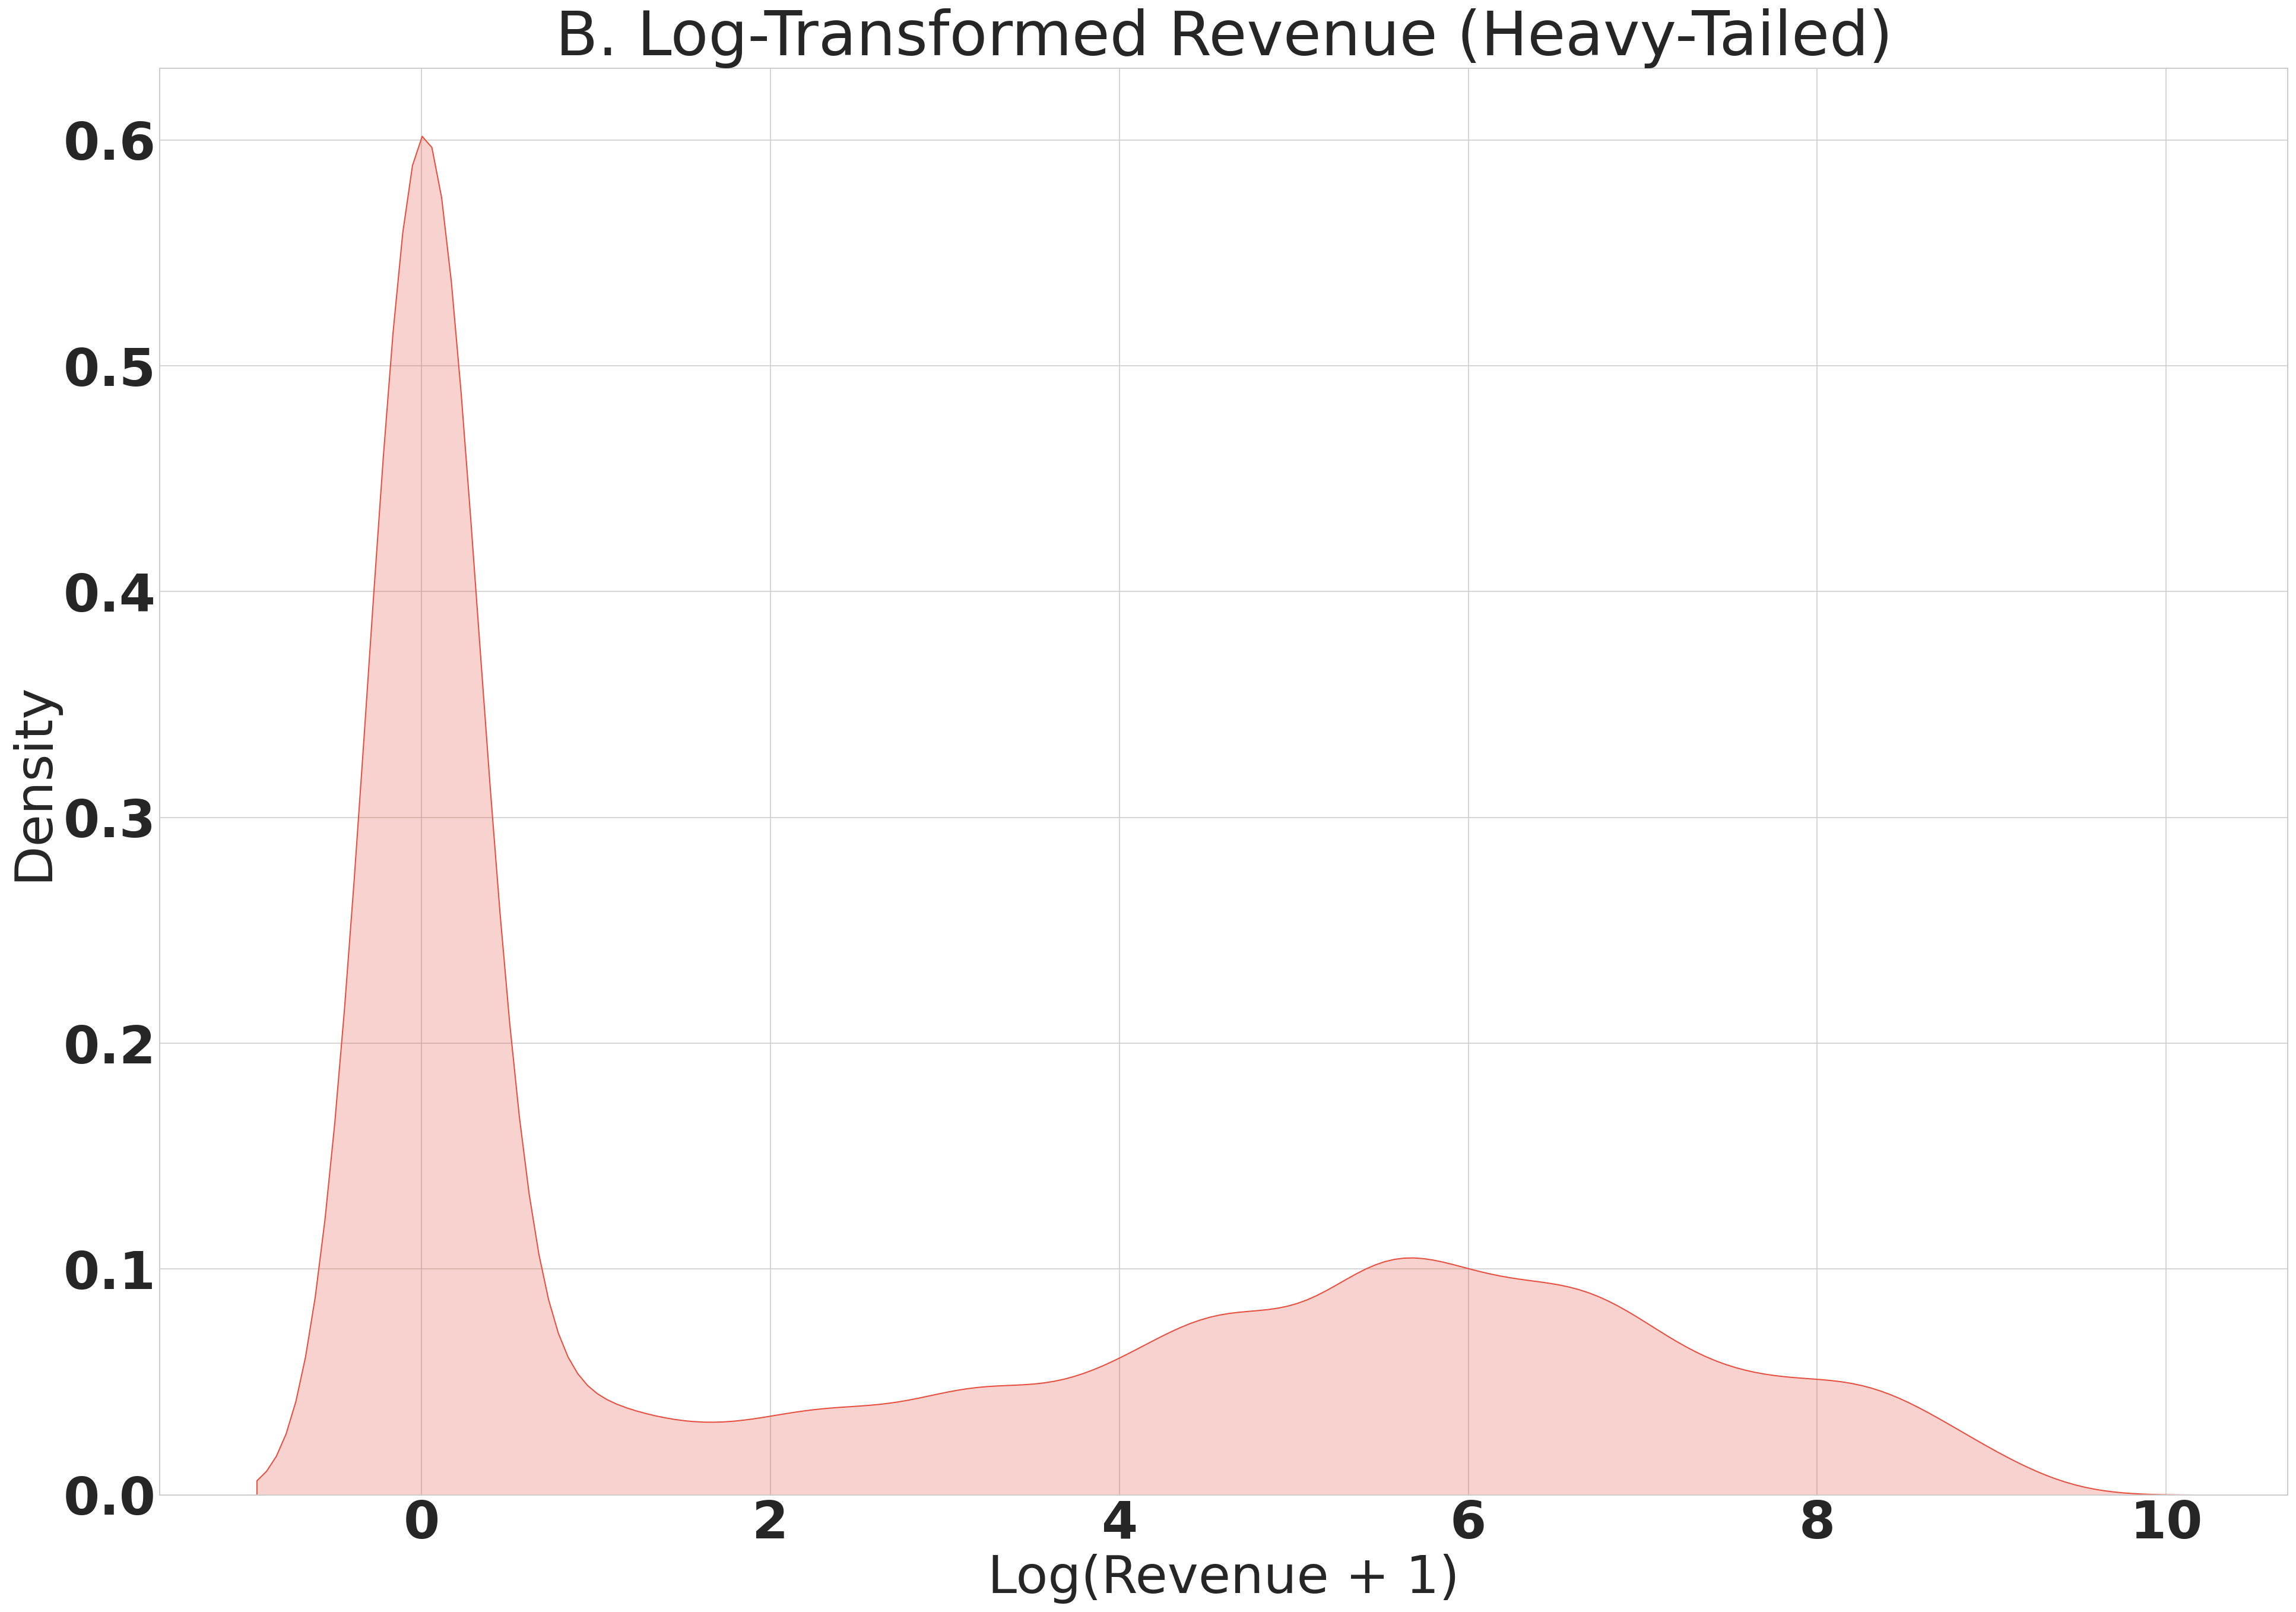
\includegraphics[width=0.25\textwidth]{revenue_plot_2.png}
%     \caption{\textbf{The Zero-Mass Distributional Challenge.} (A) The raw distribution of B2B incremental revenue is dominated by a massive spike at zero (``Zero-Mass''), accounting for $>80\%$ of the population. Standard MSE losses minimize global error by collapsing predictions toward this zero mean, failing to identify potential lift. (B) The log-transformed view reveals a heavy-tailed positive distribution, confirming that revenue follows a Zero-Inflated LogNormal (ZILN) mixture rather than a standard Gaussian \cite{rerum2024}.}
%     \label{fig:zero_mass_dist}
% \end{figure*}

% \begin{figure}[h]
%     \centering
%     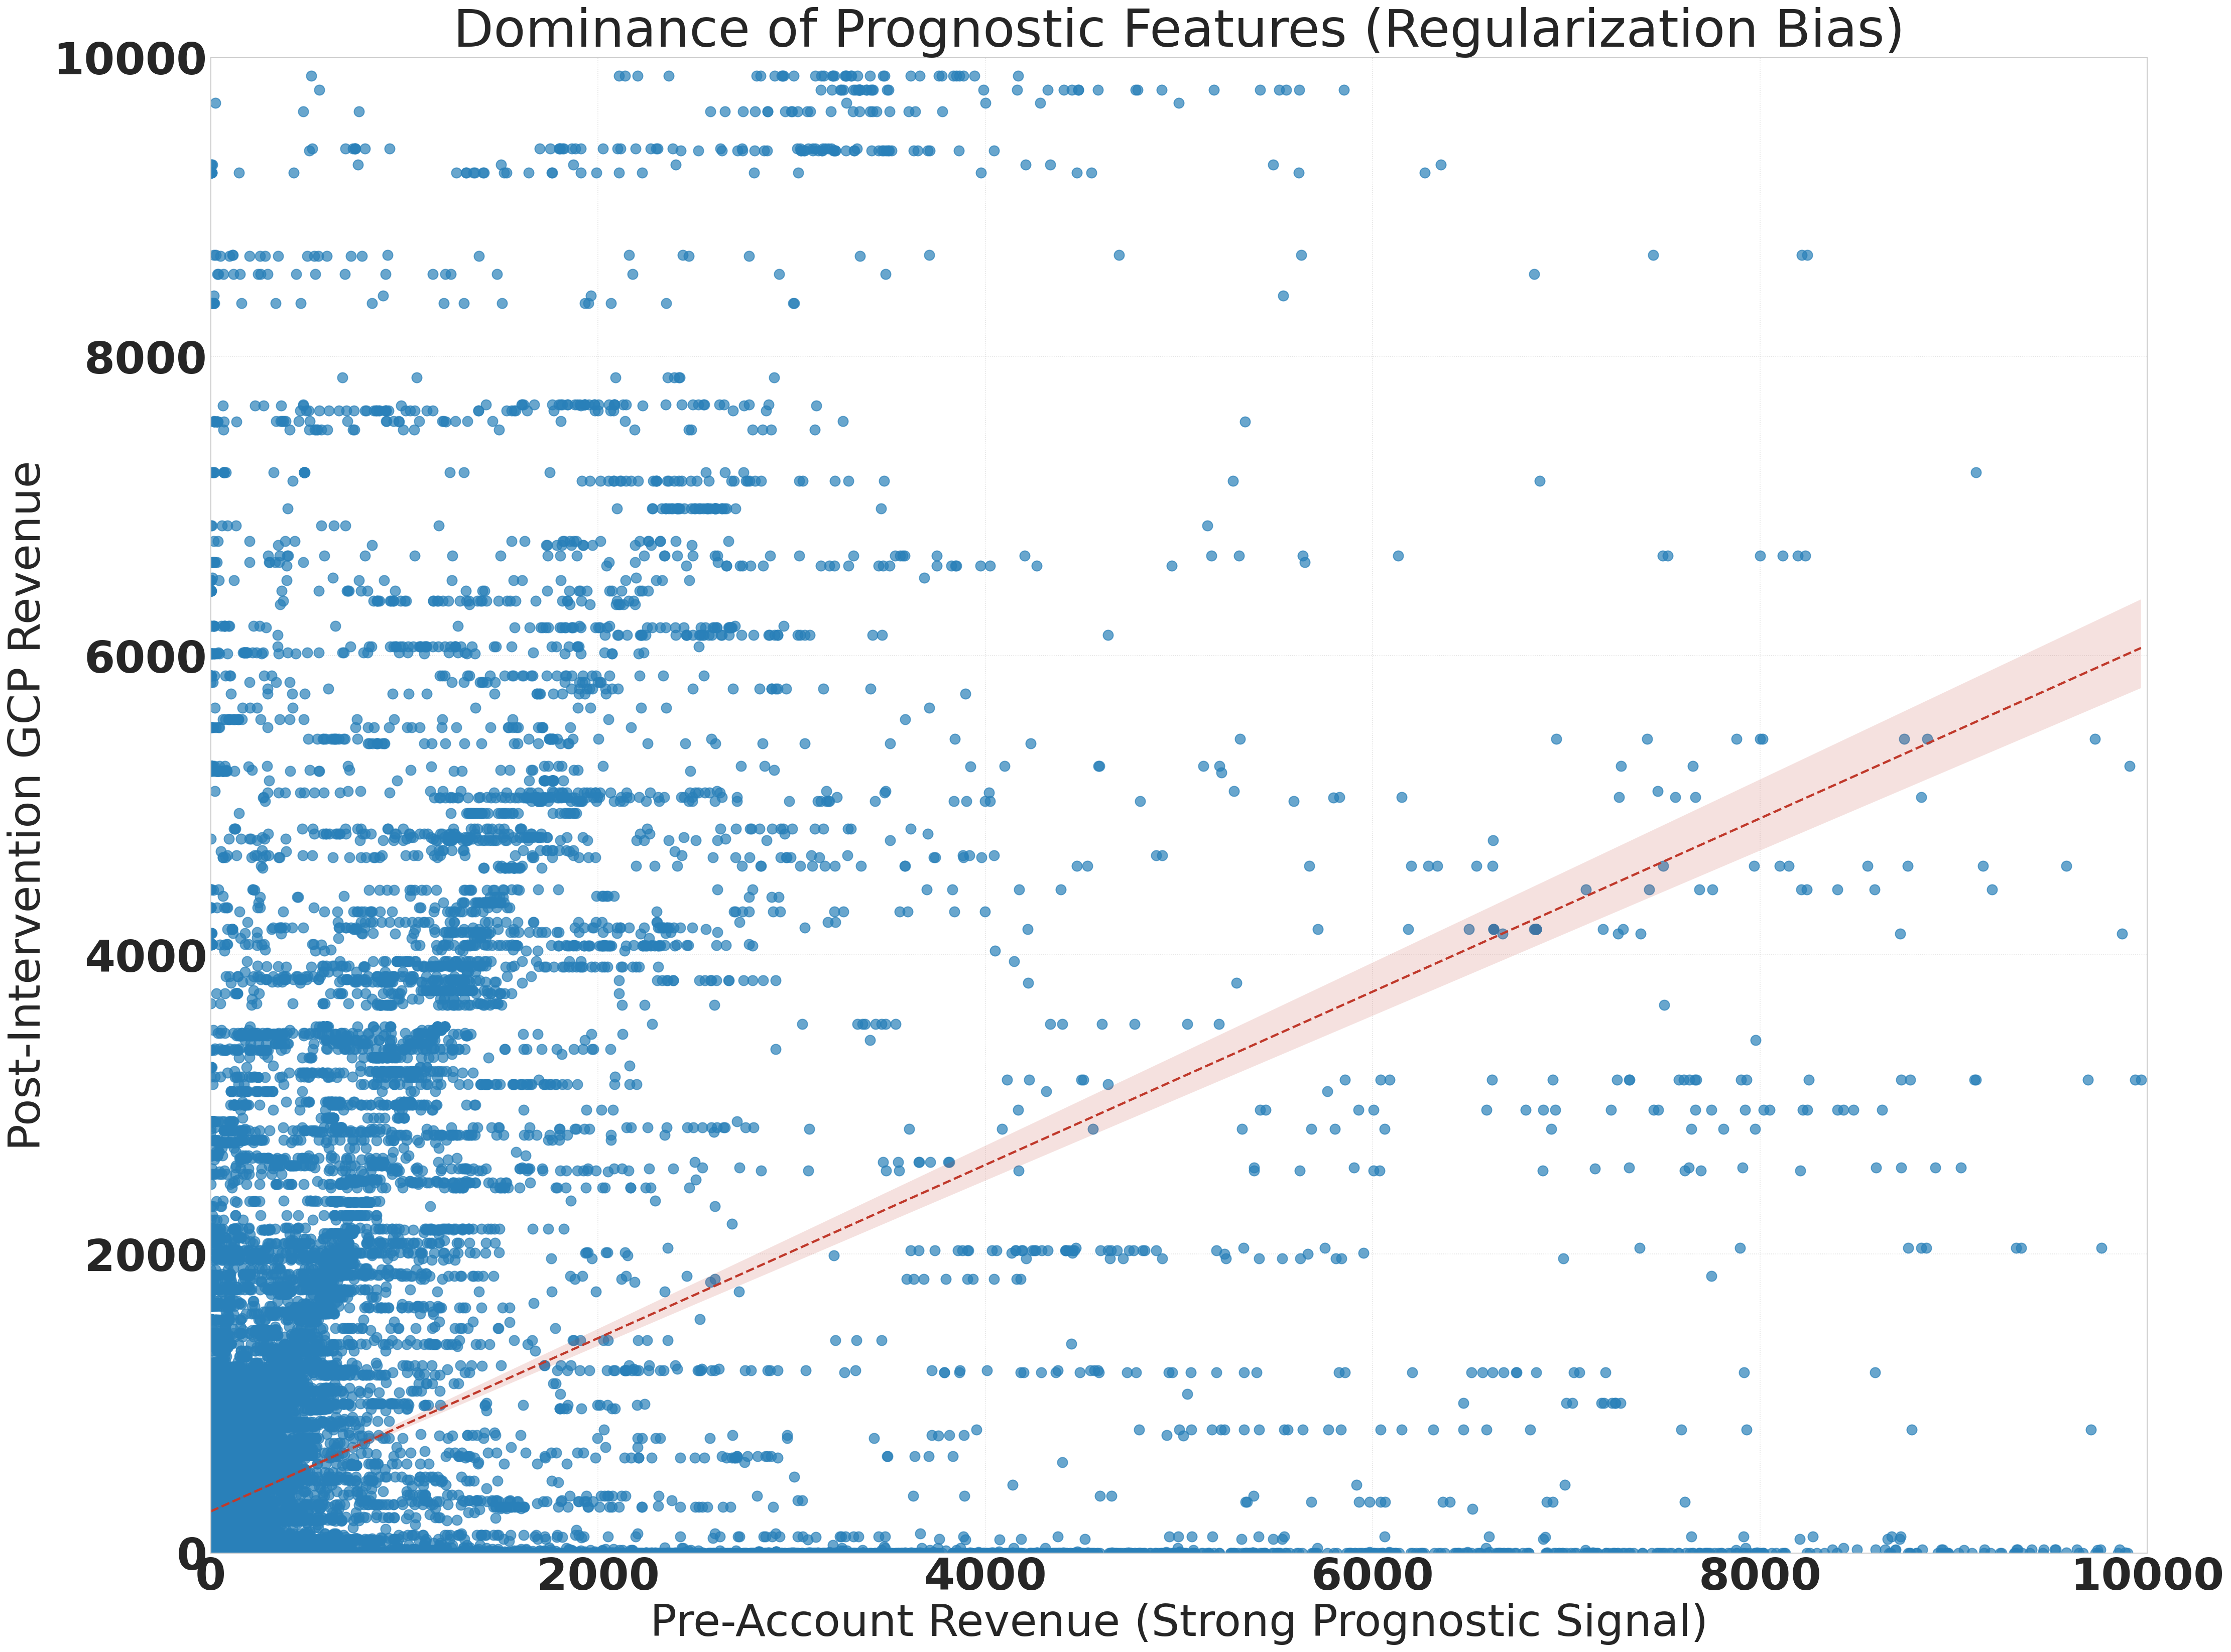
\includegraphics[width=0.75\linewidth]{vanishing_treatment.png}
%     \caption{\textbf{Prognostic Dominance and the Vanishing Treatment.} The strong linear correlation between pre-existing account revenue (x-axis) and post-intervention revenue (y-axis) illustrates the ``Regularization Bias'' challenge. In high-dimensional spaces, deep learning models prioritize these strong prognostic main effects over the subtle, heterogeneous treatment effects, effectively causing the CATE estimate to collapse to zero \cite{efin2023, shalit2017estimating}.}
%     \label{fig:prognostic_bias}
% \end{figure}


\end{document}